\section{PyTorch 简介}
\subsection{主流深度学习框架}
\begin{figure}[!h]
  \centering
  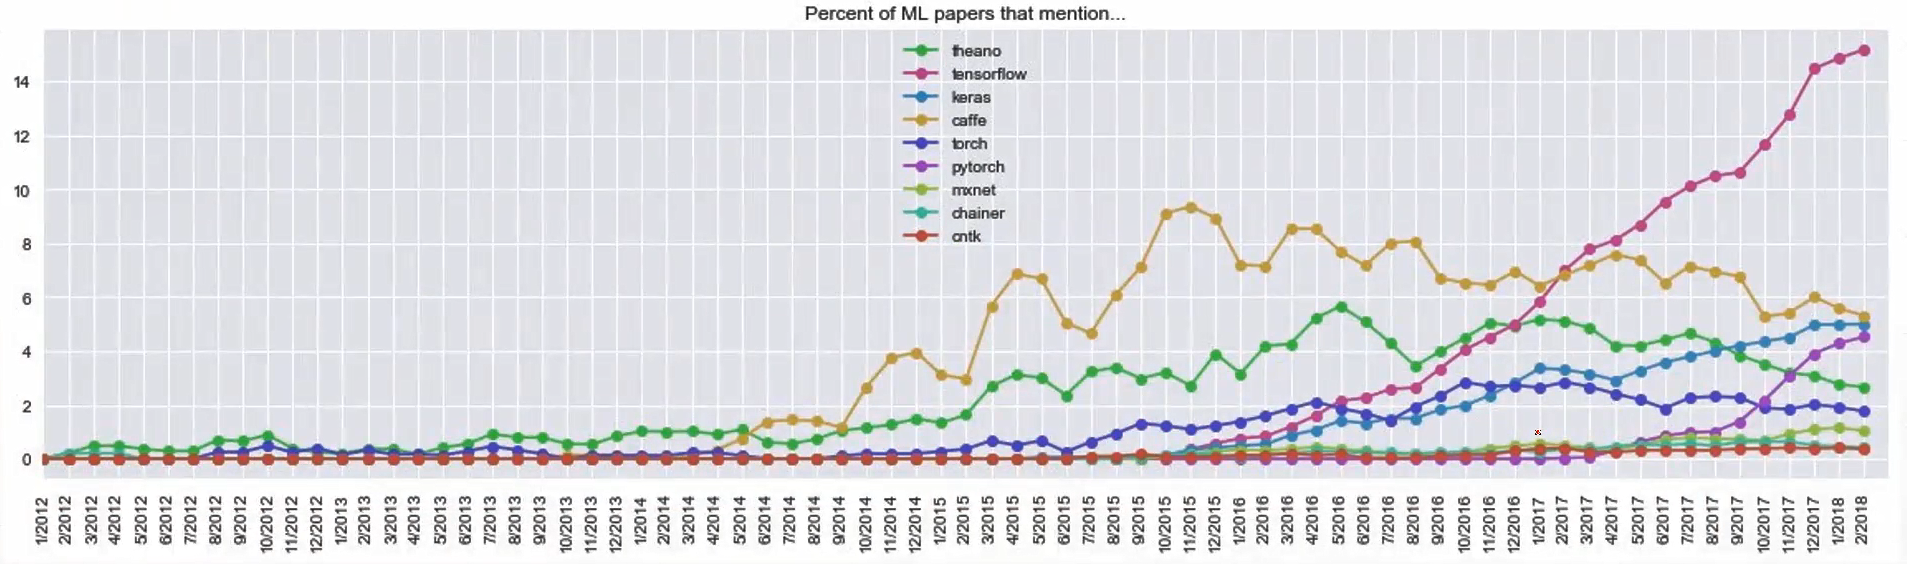
\includegraphics[width=1.02\textwidth]{trade.png}
\end{figure}

\subsection{两类深度学习框架的优缺点}
\begin{enumerate}
  \item 动态图(PyTorch)\\
  计算图的进行与代码的运行时同时进行的。
  \item 静态图(TensorFlow)【* TensorFlow 2.0 动态图优先】
  \begin{enumerate}
    \item 自建命名体系
    \item 自建时序控制
    \item 难以介入
  \end{enumerate}
\end{enumerate}

\subsection{使用深度学习框架的优点}
\begin{enumerate}
  \item GPU 加速  (cuda)
  \item 自动求导
  \item 常用网络层的API\\

\end{enumerate}

\subsection{PyTorch 的特点}
\begin{enumerate}
  \item 支持 GPU
  \item 动态神经网络
  \item Python 优先
  \item 命令式体验
  \item 轻松扩展
\end{enumerate}

\section{安装环境准备}
\begin{enumerate}
  \item 操作系统选择 (Windows Linux MacOS) 均可
  \item Python 开发环境安装 (Anaconda)
  \item PyTorch 安装
  \begin{enumerate}
    \item 安装 Nvidia Cuda
    \item 安装 CuDNN
    \item 安装 GPU 版本的 PyTorch
    \item 测试
  \end{enumerate}
\end{enumerate}

配置环境:windows10,NVIDIA GEFORCE GTX 950M

具体安装过程:
\begin{enumerate}
  \item 更新 nvidia 驱动
  \item CUDA10 安装 (采用网络安装)
  \item cuDNN7 安装 (解压配置系统变量)
  \item Pytorch 安装 (阿里源 conda安装)
  \item 测试
\end{enumerate}


\section{初见深度学习}

\begin{enumerate}
  \item 梯度下降算法 (Gradient Decent) 深度学习的精髓。
  \item 线性回归的损失函数 $Loss=(w^Tx+b-y)^2$。
  \item 利用梯度下降进行 最小化损失函数迭代工作(平均梯度信息)。
  \item 引入手写字体识别问题(MNIST)。 \\线性嵌套 非线性映射 ReLu。
\end{enumerate}





\newpage

\section{PyTorch 张量操作}

\subsection{基本数据类型}
\begin{enumerate}
  \item Python PyTorch 数据类型对比
\begin{figure}[!h]
  \centering
  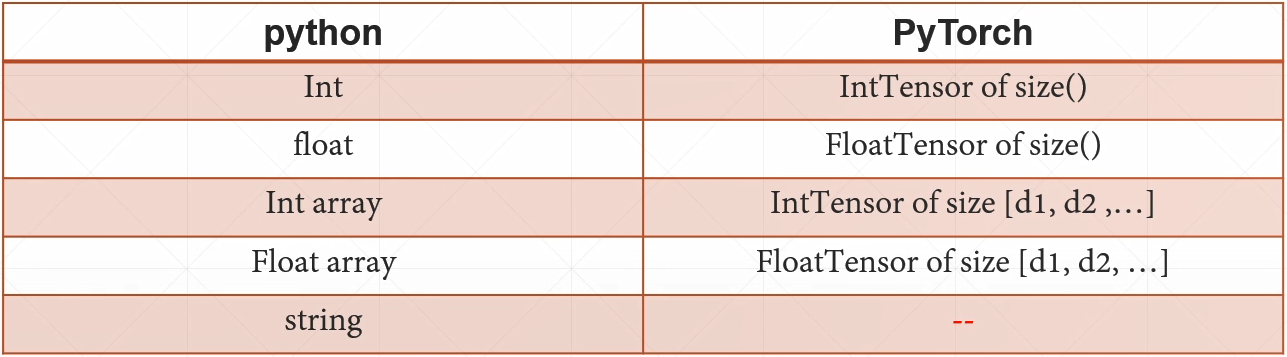
\includegraphics[width=0.98\textwidth]{PythonPyTorchDataType.png}
\end{figure}
  \item PyTorch 是面向数值计算的 GPU 加速库,没有内建对 str 类型的支持。
  \begin{enumerate}
    \item one-hot   $[0,1,0,0,\cdots]$
    \item Embedding(常用的编码语言[NLP])
    \begin{enumerate}
      \item word2vec
      \item glove
    \end{enumerate}
  \end{enumerate}
  \item PyTorch 内建的数据类型
\begin{figure}[!h]
  \centering
  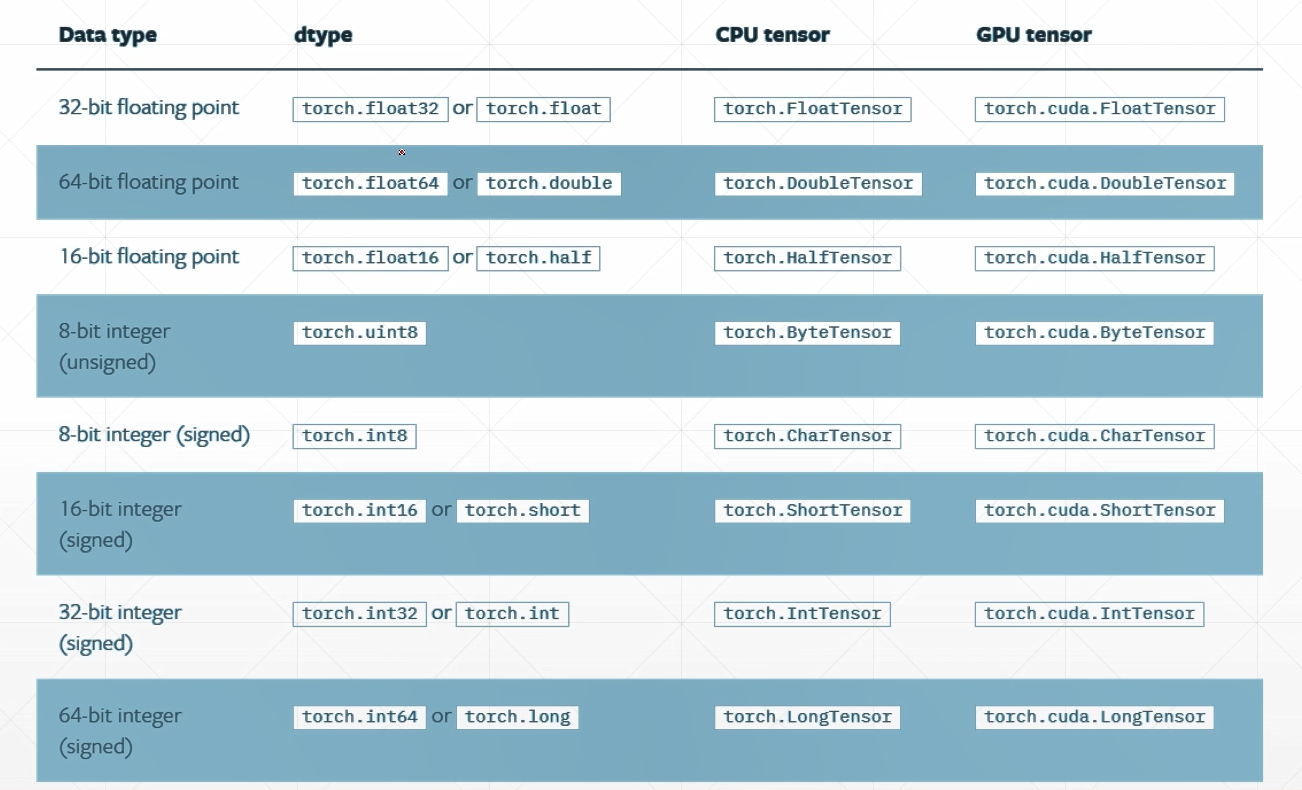
\includegraphics[width=1\textwidth]{PyTorchDataType.png}
\end{figure}
  \item PyTorch 基本数据类型
    \begin{enumerate}
      \item 标量   (0维)    \\ 一维长度为1的张量确实也可以表示张量 \\为了语义更清晰,在版本PyTorch0.3之后,两个概念从形式上加以区分,并增加了长度为零的 tensor。
      \item 张量   (1维)     Bias or Linear input  (单张图片输入)
      \item 张量   (2维)     Linear input batch  (多张图片输入)
      \item 张量   (3维)     RNN input Batch (循环神经网络批量输入) \newline[word,sentence,feature]
      \item 张量   (4维)     CNN input Batch (卷积神经网络批量输入)  \newline [batch,channel,height,width]    'r','g','b'三原色通道
    \end{enumerate}
  \item 区分 dim  size  shape  tensor
  \begin{enumerate}
    \item dim :表示的是 rank。
    \item size(shape) :表示的是多少行,多少列,$\cdots$。
    \item tensor :表示具体的数据。
  \end{enumerate}
\end{enumerate}


\subsection{创建 Tensor}

\begin{enumerate}
  \item import from numpy
  \begin{lstlisting}
  torch.from_numpy()
  \end{lstlisting}

  \item import from list
  \begin{lstlisting}
  torch.tensor()   #data
    torch.tensor([1., 2.])
  torch.Tensor()   #data or shape(size)  == torch.FloatTensor()
    torch.Tensor([1., 2.]) #No use as far as possible
    torch.Tensor(2, 3)
  \end{lstlisting}

  \item uninitialized (未初始化的(有隐患 极大 与 极小)) \\
  使用未初始化的数据一定要覆盖,否则可能会出现非常大或者非常小的数据。\\
  导致出现 torch.non or torch.inf 的 bug。
  \begin{lstlisting}
  torch.empty() #shape
  torch.Tensor()
  torch.IntTensor()
  torch.FloatTensor()
  \end{lstlisting}

  \item set defalt type (设置默认的 tensor 数据类型)
  \begin{lstlisting}
  In [61]:  torch.tensor([1.2, 3]).type()
  Out[61]: 'torch.DoubleTensor'

  In [62]:  torch.set_default_tensor_type(torch.FloatTensor)

  In [63]:  torch.tensor([1.2, 3]).type()
  Out[63]: 'torch.FloatTensor'
  \end{lstlisting}

  \item 随机初始化 (rand/rand\_like, randint)
  \begin{lstlisting}
  rand()                      input : shape [0,1]
  randint(min,max,[shape])    [min,max)
  rand_like()                 input : tensor
  randn()                     input : shape       data ~ N(0,1)
    torch.normal(mean=torch.full([10], 0), std=torch.arange(1, 0, -0.1))
  \end{lstlisting}

  \item 初始化为同一个数 (也可以是标量)
  \begin{lstlisting}
  torch.full([shape],number)
  \end{lstlisting}

  \item 生成递增递减序列
  \begin{lstlisting}
  arange/range          int
  torch.arange(0, 10)          #[0, 10)
  torch.arange(0, 10, 2)
  torch.arange(10, 0, -1)
  torch.range(0, 10)           #[0, 10] no use as far as possible

  linspace/logspace    float
  torch.linspace(0, 10, steps=4)     #four numbers
  torch.logspace(-1, 0, steps=10)    #10^n
  \end{lstlisting}

  \item ones/zeros/eyes
  \begin{lstlisting}
  torch.ones()      #shape
  torch.zeros()     #shape
  torch.eye()       #shape        no more parameters
  torch.*_like()    #tensor
  \end{lstlisting}

  \item randperm \\
  生成随机种子 功能类似于 rondom.shuffle 随机打散 进行二元对应。
  \begin{lstlisting}
  In : torch.randperm(10)
  Out: tensor([0, 1, 4, 8, 2, 9, 5, 6, 3, 7])
  \end{lstlisting}
\end{enumerate}


\subsection{索引和切片}
\begin{enumerate}
  \item indexing
  \begin{lstlisting}
  a = torch.rand(10,3,28,28)
  a[0].shape)  #'第0张照片'
  a[0,0].shape  #'第0张照片的第0个通道'
  a[0,0,0].shape #'第0张照片的第0个通道的第0行像素   dim为1'
  a[0,0,0,0]  #'第0张照片的第0个通道的第0行的第0个像素 dim为0'
  \end{lstlisting}

  \item select first/last N/by step
  \begin{lstlisting}
  a[:2].shape   #'取前两张图片'
  a[-2:].shape  #'取后两张图片'

  a[:2,:1].shape   #'取前两张图片的第一个通道'
  a[-2:,-2:].shape  #'取后两张图片的后两个通道'

  a[:,:,0:28:2,0:28:2].shape   #'取全部图片的全部通道的长宽均间隔采样'
  \end{lstlisting}

  \item select by specific index
  \begin{lstlisting}
  a[2][1][18][26]  #'取第2张图片的第1通道的第18行26列的像素值, 标量'
  a.index_select(dim,tensor)    #'第一个参数表示维度,  第二个是tensor值'
  a.index_select(0,torch.tensor([0, 3, 3])) #'选择第0第3第3张图片'
  a.index_select(1,torch.tensor([0,2]))  #'选择四张图片的第0和第2的通道'
  a.index_select(2,torch.arange(0,8))  #'选择四张图片每个通道的前8所有列的像素'
  \end{lstlisting}

  \item 符号 ... (选取足够多的维度  可推测而省略:号)
  \begin{lstlisting}
  a[...].shape
  a[:3,...].shape
  a[:,1,...].shape
  a[...,:10].shape
  a[0,...,::2].shape  #'间隔采样 ::'
  \end{lstlisting}

  \item select by mask (依据掩码的位置信息索引)
  \begin{lstlisting}
  x = torch.randn(3,3)
  mask = x.ge(0.5)  #'>=0.5 的位置信息 '
  torch.masked_select(x,mask)  #'得到所有>=0.5的tensor值'
  \end{lstlisting}

  \item select by flatten index (打平索引)
  \begin{lstlisting}
  src = torch.tensor([[1,2,3], [4,5,6]])
  torch.take(src, torch.tensor([0,2,5])).shape     #torch.Size([3])
  torch.index\_select()   '类似torch.take 但是未打平'
  \end{lstlisting}
\end{enumerate}


\subsection{Tensor 维度变换}
Tensor 常用API
\begin{enumerate}
  \item View/reshape (不增加数据和减少数据)
  \begin{lstlisting}
  a = torch.rand(4, 1, 28, 28)
  a.shape   #'torch.Size([4, 1, 28, 28])'
  a.view(4,28, 28)   #'torch.Size([4, 28, 28])'
  a.reshape(4, 28*28).shape   #'torch.Size([4, 784])'     '全链接层'
  a.reshape(4*28, 28)
  '存在问题, 丢失维度逻辑信息,数据污染'
  b = a.reshape(4, 28*28)
  b.reshape(4,1,28,28)
  \end{lstlisting}

  \item Squeeze(删减维度)/unsqueeze(增加维度)
\begin{figure}[!h]
  \centering
  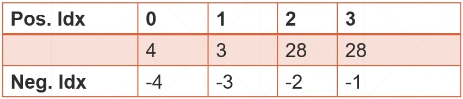
\includegraphics[width=0.75\textwidth]{unsqueeze.png}
\end{figure}
  \begin{lstlisting}
  #unsqueeze   '维度增加'
  '尽量不要用负数' '(不增加数据和减少数据)   插入范围 [-a.dim-1, a.dim+1)'
  a.shape   #torch.Size([4, 1, 28, 28])
  a.unsqueeze(0).shape   #[1, 4, 1, 28, 28]   '0维度前面插入一个维度'
  a.unsqueeze(-1).shape   #[4, 1, 28, 28, 1]   '在最后一个维度后面插入一个维度'
  a.unsqueeze(4).shape   #[4, 1, 28, 28, 1]
  a.unsqueeze(-5).shape   #[1, 4, 1, 28, 28]
  \end{lstlisting}
  \begin{lstlisting}
  '维度增加例子'
  a = torch.tensor([1.125,2.258])
  a,     #tensor([1.1250, 2.2580])
  a.shape,   #torch.Size([2])
  a.unsqueeze(1),   #tensor([[1.1250],[2.2580]])
  a.unsqueeze(1).shape   #torch.Size([2, 1])
  a.unsqueeze(0),   #tensor([[1.1250, 2.2580]])
  a.shape,   ##torch.Size([1, 2])
  \end{lstlisting}
  \begin{lstlisting}
  '为了实现 a+b 先维度增加 unqueeze, 在相关维度扩展后相加'
  b = torch.rand(32)
  a = torch.rand(4,32,16,16)
  b = b.unsqueeze(1).unsqueeze(2).unsqueeze(0)
  b.shape    #torch.Size([1, 32, 1, 1])
  \end{lstlisting}
  \begin{lstlisting}
  #squeeze '压缩/挤压'
  a = torch.rand(1, 32, 1, 1)
  a.squeeze().shape  #torch.Size([32])   '尽可能多的删减维度'
  a.squeeze(0).shape   #torch.Size([32, 1, 1])
  a.squeeze(-2).shape   #torch.Size([1, 32, 1])
  a.squeeze(1).shape   #torch.Size([1, 32, 1, 1])   '维度不变'
  \end{lstlisting}

  \item Transpose(单次交换)/t/permute(多次交换)(维度交换)
  \begin{lstlisting}
  a = torch.randn(3,4)
  a.t()   '只能适用于二维转置'
  \end{lstlisting}
  \begin{lstlisting}
  a = torch.randn(4, 3, 28, 28)  '记录维度信息否则污染数据'
  b = a.transpose(1,3).reshape(4, 3*28*28).reshape(4, 3, 28, 28)   '数据污染'
  c = a.transpose(1,3).reshape(4, 3*28*28).reshape(4, 28, 28, 3)   .transpose(1,3)
  torch.all(torch.eq(a, b))   #tensor(0, dtype=torch.uint8)
  torch.all(torch.eq(a, c))   #tensor(1, dtype=torch.uint8)
  \end{lstlisting}
  \begin{lstlisting}
  transpose '只能做单次交换 '  '但' permute '可以做多次交换'
  a = torch.randn(4, 3, 28, 32)     '目标(4, 28, 32, 3)'
  a.transpose(1, 3).transpose(1, 2).shape   #torch.Size([4, 28, 32, 3])
  a.permute(0, 2, 3, 1).shape   #torch.Size([4, 28, 32, 3])
  \end{lstlisting}

  \item Expend/repeat (维度扩展)\\
  Expand: broadcasting 推荐使用, 内存无关, 节约内存。\\
  Repeat: memory copied  内存相关。
  \begin{lstlisting}
  #rexpand '表示扩展到的维度'
  b = torch.rand(1, 32, 1, 1)  '维度元素才可expand, repeat没有此条限制'
  b.expand(4, 32, 16, 16).shape   #torch.Size([4, 32, 16, 16])
  b.expand(-1, 32, 16, 16).shape   #torch.Size([1, 32, 16, 16])
  b.expand(-1, 32, -1, -4).shape   #torch.Size([1, 32, 1, -4])   -4 bug '无意义'
  #repeat  '表示复制次数'
  b.repeat(4, 1, 16, 16).shape   #torch.Size([4, 32, 16, 16])
  b.repeat(4, 2, 16, 16).shape   #torch.Size([4, 64, 16, 16])
  \end{lstlisting}
\end{enumerate}





\newpage
\section{张量高阶操作}
\subsection{Broadcast}
Broadcast  (expand+withoutcopying) [广播机制]
\begin{figure}[!h]
  \centering
  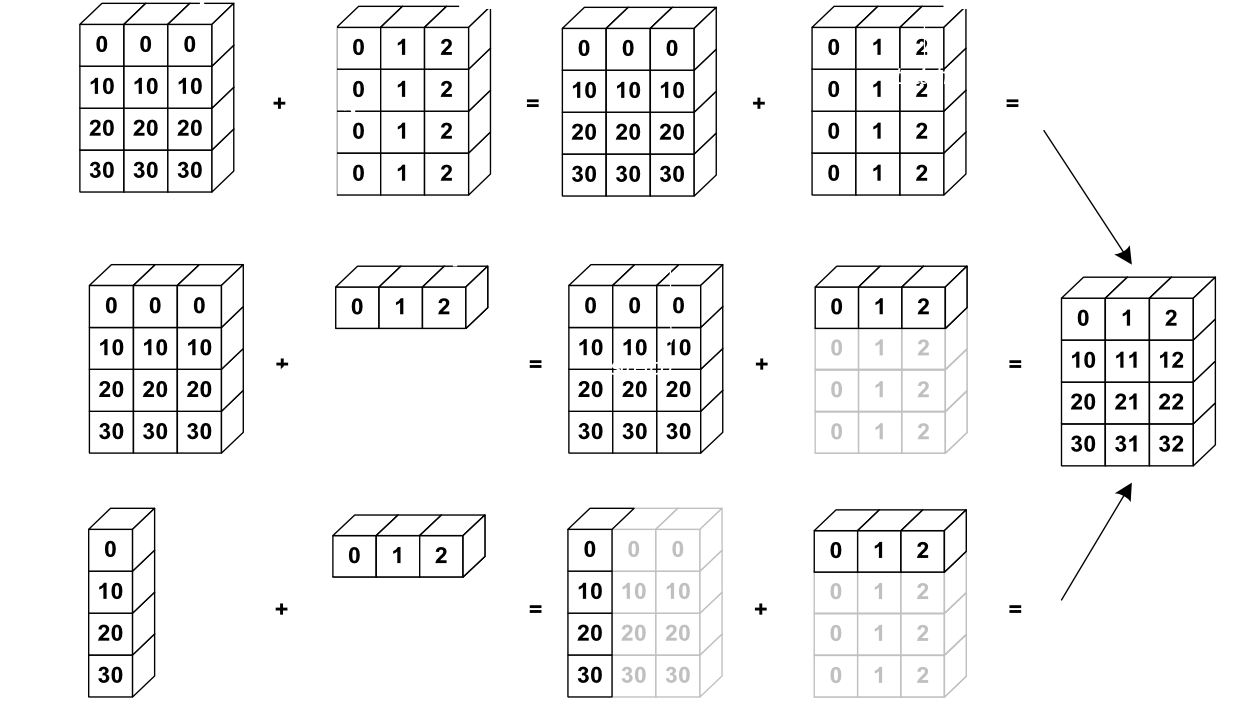
\includegraphics[width=0.8\textwidth]{broadcasting.png}
\end{figure}

    关键步骤:
    \begin{enumerate}
      \item Insert 1 dim ahead  (unsqueeze)
      \item Expand dims with size 1 to same size
      \item Feature maps: [4, 32, 14, 14]
      \item Bias: [32, 1, 1] =$>$ [1, 32, 1, 1] =$>$ [4, 32, 14, 14]
    \end{enumerate}

    存在意义:
    \begin{enumerate}
      \item for actual demanding(实际需求)
      \begin{itemize}
        \item $[class, students, scores]$
        \item $Add bias for every students: +5 score$
        \item $[4, 32, 8] + [4, 32, 8]$
        \item $[4, 32, 8] + [5.0]$
      \end{itemize}
      \item memory consumption(节约内存)
      \begin{itemize}
        \item $[4, 32, 8] => 1024$
        \item $[5.0] => 1 $
      \end{itemize}
    \end{enumerate}

    使用环境:  match from last dim
    \begin{enumerate}
      \item If current dim=1, expand to same
      \item If either has no dim, insert one dim and expand to same
      \item otherwise, NOT broadcasting-able
    \end{enumerate}

    具体案例:
    \begin{enumerate}
      \item Situation 1
      \begin{itemize}
        \item $[4, 32, 14, 14]$
        \item $[1, 32, 1, 1] => [4, 32, 14, 14]$
      \end{itemize}
      \item Situation 2
      \begin{itemize}
        \item $[4, 32, 14, 14]$
        \item $[14, 14] => [1, 1, 14, 14] => [4, 32, 14, 14]$
      \end{itemize}
      \item Situation 3
      \begin{itemize}
        \item $[4, 32, 14, 14]$
        \item $[2, 32, 14, 14] => error$
      \end{itemize}
    \end{enumerate}

\begin{lstlisting}
a = torch.rand(1,3)
b = torch.rand(3,1)
(a+b).shape   #torch.Size([3, 3])
a = torch.rand(4, 32, 14, 14)
b = torch.rand(1, 32, 1, 1)
(a+b).shape   #torch.Size([4, 32, 14, 14])
a = torch.rand(4, 32, 14, 14)
b = torch.rand(14, 14)
(a+b).shape   #torch.Size([4, 32, 14, 14])
a = torch.rand(4, 32, 14, 14)
b = torch.rand(2, 32, 14, 14)
(a+b).shape   error
(a+b[0]).shape  #torch.Size([4, 32, 14, 14])   '手动指定'
a = torch.rand(2, 3, 6, 6)
b = torch.rand(1, 3, 6, 1)   '给每一个通道的每一行加上相同的像素值'
(a+b).shape
\end{lstlisting}

\subsection{Tensor 分割与合并}
Tensor 分割与合并(Merge or splite)
\begin{enumerate}
  \item Cat 合并 , 不增加维度,cat维度可以不同。
  \begin{lstlisting}
  a = torch.rand(4, 32, 8)   #[classes, students, scores]
  b = torch.rand(5, 32, 8)
  torch.cat([a, b],dim=0).shape   #torch.Size([9, 32, 8])
  \end{lstlisting}
  \item Stack 合并, 创建新的维度,旧维度必须一致。
  \begin{lstlisting}
  a = torch.rand(32, 8)  #[students, scores]
  b = torch.rand(32, 8)
  c = torch.rand(32, 8)
  torch.stack([a, b, c],dim=0).shape   #torch.Size([3, 32, 8])
  \end{lstlisting}
  \item Split 根据长度来拆分。
  \begin{lstlisting}
  a = torch.rand(4, 32, 8)      #[classes,  students, scores]
  aa, bb, cc = a.split([1,2,1], dim=0)
  aaa, bbb = a.split(2, dim=0)
  aa.shape   #torch.Size([1, 32, 8])
  bb.shape   #torch.Size([2, 32, 8])
  cc.shape   #torch.Size([1, 32, 8])
  aaa.shape   #torch.Size([2, 32, 8])
  bbb.shape   #torch.Size([2, 32, 8])
  \end{lstlisting}
  \item Chunk  根据数量来拆分。
  \begin{lstlisting}
  a = torch.rand(6, 32, 8)      #[classes, students, scores]
  aa, bb= a.chunk(2, dim=0)
  cc, dd, ee =a.split(2, dim=0)
  aa.shape   #torch.Size([3, 32, 8])
  bb.shape   #torch.Size([3, 32, 8])
  cc.shape   #torch.Size([2, 32, 8])
  dd.shape   #torch.Size([2, 32, 8])
  ee.shape   #torch.Size([2, 32, 8])
  \end{lstlisting}
\end{enumerate}

\subsection{Tensor 运算}
tensor 矩阵的基本运算
\begin{enumerate}
  \item Add/minus/multiply/divide
  \begin{lstlisting}
  a = torch.rand(4,3)
  b = torch.rand(3)
  torch.all(torch.eq(a+b, torch.add(a,b)))   #tensor(1, dtype=torch.uint8)
  a-b   #torch.sub
  a*b   #torch.mul
  a/b   #torch.div
  a//b  '地板除'
  \end{lstlisting}
  \item Matmul   \\最后两维做矩阵乘运算,其他符合broadcast机制
  \begin{lstlisting}
  a = torch.rand(4,3)
  b = torch.rand(3,8)
  torch.mm(a, b)   #only for 2d
  (a @ b).shape   #torch.matmul  torch.Size([4, 8])
  \end{lstlisting}
  \item Pow
  \begin{lstlisting}
  a**2   #torch.pow
  \end{lstlisting}
  \item Sqrt/rsqrt/exp/log \\平方根/平方根的倒数/自然常数幂/自然常数底
  \begin{lstlisting}
  a.sqrt()   #a**0.5
  a.rsqrt()
  torch.exp(a)   #e**a
  \end{lstlisting}
  \item Round 近似运算
  \begin{lstlisting}
  a = torch.tensor(3.14)   #tensor(3.14)
  a.floor(), a.ceil(), a.round()   #tensor(3.) tensor(4.) tensor(3.)
  a.trunc()   #tensor(3.)
  a.frac()   #tensor(0.1400)
  \end{lstlisting}
  \item clamp 数字裁剪  \\
  使用环境   '梯度裁剪'\\ 梯度弥散(梯度非常小 $<0.*$),梯度爆炸(梯度非常大 $>*00$)\\
  打印梯度的 L2 范数观察  (W.grad.norm(2))\\
  \begin{lstlisting}
  grad = torch.rand(3,4)*15
  grad.min()   #min number
  grad.max()   #max number
  grad.median()   #medoan number
  grad.clamp(10)  #min number is 10
  grad.clamp(0, 10)   #all numbers is [0,10]
  \end{lstlisting}
\end{enumerate}

\subsection{Tensor 统计}
\begin{enumerate}
  \item norm\\
  表示范数,不同于 normalize(正则化)
  \begin{align*}
  &\text{~vector ~~norm}   &\text{matrix~~ norm~~~~~~~~~~}\\
  &||x||_1 = \sum_{i=1}^{n}|a_i| &||A||_1=\max\limits_{i\le j \le n}\sum_{i=1}^{n}|a_{ij}|\\
  &||x||_e = \sqrt{\sum_{i=1}^{n}x_i^2}   &||A||_e=\sqrt{\sum_{i=1}^{n}\sum_{j=1}^{n}a_{ij}^2}\\
  &||x||_p = \Big(\sum_{i=1}^{n}|x_i|^p\Big)^{\frac{1}{p}}  &||A||_p=\Big(\sum_{i=1}^{n}\sum_{j=1}^{n}a_{ij}^2\Big)^{\frac{1}{p}}\\
  \end{align*}
  \begin{lstlisting}
  a = torch.full([8], 1)
  b = a.reshape(2, 4)
  c = b.reshape(2, 2, 2)
  a   #tensor([1., 1., 1., 1., 1., 1., 1., 1.])
  b   #tensor([[1., 1., 1., 1.], [1., 1., 1., 1.]])
  a.norm(1), b.norm(1), c.norm(1)   #tensor(8.)
  a.norm(2), b.norm(2), c.norm(2)   #tensor(2.8284)
  #two parameters norm, dimension
  a.norm(1, dim=0)   #tensor(8.)
  b.norm(1, dim=1)   #tensor([4., 4.])
  c.norm(2, dim=2)   #tensor([[1.4142, 1.4142], [1.4142, 1.4142]])
  \end{lstlisting}

  \item max, min, mean, sum, prod(累乘)
  \begin{lstlisting}
  a = torch.arange(8).reshape(2,4).float()
  a.min()   #tensor(0.)
  a.max()   #tensor(7.)
  a.mean()   #tensor(3.5)
  a.mean(1)   #tensor([1.5000, 5.5000])
  a.sum()   #tensor(28.)
  a.prod()   #tensor(0.)
  \end{lstlisting}

  \item  argmin, argmax(参数 dim, keepdim)
  \begin{lstlisting}
  a = torch.randn(4, 10)  '4张照片 0-9 10个概率值'
  a.argmin() a.argmax()  '无参数默认打平'
  a.argmax(1)   '返回每张照片概率最大的数字'
  a.argmax(1, keepdim=True)   '返回每张照片概率最大的数字并保持维度信息'
  a.'max'(1)  '返回每张照片最大的概率及数字'
  \end{lstlisting}

  \item Kthvalue, topk(比 max 返回更多的数据)
  \begin{lstlisting}
  a = torch.randn(4, 10)  '4张照片 0-9 10个概率值'
  a.topk(2, dim=1, largest=True))  'largest = False 表示最小的 k 个'
  a.kthvalue(10, dim=1)   '返回第10小的概率及位置'
  \end{lstlisting}

  \item compare (比较操作)\\
  $>, <, >=, <=, !=, ==$\\
  torch.eq()   ~~~~~~可 braodcast, 返回 0/1 同型\\
  torch.equal()   ~~~~~~比较每一值,都相等返回 True
\end{enumerate}


\subsection{Tensor 高阶操作}
\begin{enumerate}
  \item where  (GPU 离散复制)
  \begin{lstlisting}
  torch.where(condition, x, y) --> Tensor '满足条件取 x, 否则取 y'
  '其功能可由for 逻辑功能实现, 但运行在CPU, 难以高度并行'
  condition '必须是与 x, y 同型的1/0型'   'x, y可 broadcast'
  a = torch.rand(2, 2)
  b = torch.ones(2, 2)
  c = torch.zeros(2, 2)
  torch.where(a>0.5, b, c)
  \end{lstlisting}
  \item Gather  (GPU 收集查表操作)
  \begin{lstlisting}
  torch.gather('input', dim, index, out=None)  --> Tensor '查表操作'
  out[i][j][k] = 'input'[index[i][j][k]][j][k]   dim=0
  out[i][j][k] = 'input'[i][index[i][j][k]][k]   dim=1
  out[i][j][k] = 'input'[i][j][index[i][j][k]]   dim=2

  'Gather 查表 用来索引全局标签'
  prob = torch.rand(4, 10)   '四张图片 十个概率值'
  idx = prob.topk(3, dim=1)[1]
  label = torch.arange(10)+100
  torch.gather(label.expand(4, 10), dim=1, index=idx)
  '共四张图片 每张查概率最大的三个标签'
  \end{lstlisting}
\end{enumerate}

\section{随机梯度下降}
\subsection{梯度}
\begin{enumerate}
  \item 导数 ~~(标量)
  \item 偏微分  ~~ (函数延某个方向的变换量 ~~~ 标量)
  \item 梯度~~  (函数变化量最大的方向  ~~~向量)\\
  梯度的意义: 模为变换率大小, 矢量方向。
\begin{figure}[!h]
  \centering
  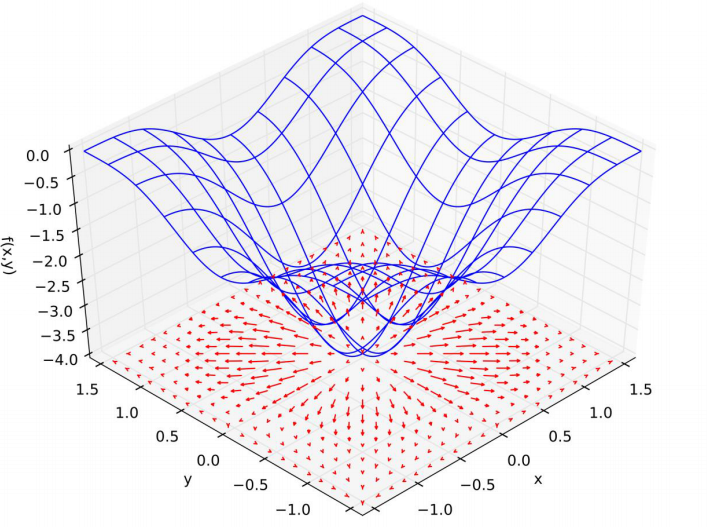
\includegraphics[width=0.75\textwidth]{gradient.png}
\end{figure}
\end{enumerate}

\textbf{如何求取最小值: 梯度下降}$$\theta_{t+1} = \theta_t-\alpha_t\nabla f(\theta_t)$$
\begin{align*}
&\text{Function}:&J(\theta_1, \theta_2)=\theta_1^2+\theta_2^2~~~~~~\\
&\text{Object}:&\min\limits_{\theta_1,\theta_2}J(\theta_1, \theta_2)~~~~~~~~~~~~\\
&\text{Update~rules}:&\theta_1:=\theta_1-\alpha\frac{d}{d\theta_1}J(\theta_1, \theta_2)\\
&~            &\theta_2:=\theta_2-\alpha\frac{d}{d\theta_2}J(\theta_1, \theta_2)\\
&\text{Derivatives}:&\frac{d}{d\theta_1}J(\theta_1, \theta_2)=2\theta_1~~~~~~\\
&~                  &\frac{d}{d\theta_2}J(\theta_1, \theta_2)=2\theta_2~~~~~~
\end{align*}

\textcolor{red}{影响优化器优化精度的两个重要因素:}
\begin{enumerate}
  \item 局部极小值
  \item 鞍点
\end{enumerate}

凸函数才会有全局最小值,通常情况下存在局部极小值。\\
(ResNet-56 论文-2018 何凯明)
\begin{figure}[!h]
  \centering
  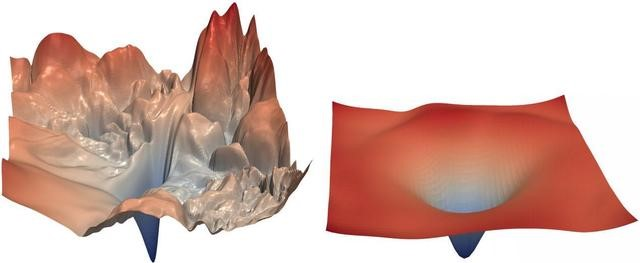
\includegraphics[width=1\textwidth]{localMinima.jpg}
\end{figure}

\textcolor{red}{影响优化器搜索过程效果的因素:}
\begin{enumerate}
  \item 初始化状态
  \item 学习率
  \item 动量(逃离局部极小值)
  \item $\cdots$
\end{enumerate}


\subsection{常见函数的梯度}
\begin{tabular}{|c|c|c|}
\hline
函数类型& 函数& 导数\\
\hline
常函数& c& 0\\
\hline
线性函数& ax& a\\
\hline
二次函数& $ax^2$&2ax\\
\hline
幂函数&$x^a$&$ax^{a-1}$\\
\hline
指数函数&$a^x$&$a^xlna$\\
~&$e^x$&$e^x$\\
\hline
对数函数&$log_a(x)$&$1/(xlna)$\\
~&lnx&1/x\\
\hline
三角函数&sin(x)&cos(x)\\
~&cos(x)&-sin(x)\\
~&tan(x)&sec(x)\\
\hline
\end{tabular}
    ~\\

\subsection{激活函数}
\textbf{1. Sigmoid/Logistic }\textcolor{red}{会伴随严重的梯度弥散现象(长时间梯度的不到更新)。}
$$f(x)=\sigma(x)=\frac{1}{1+e^{-x}}~~~~~[0,1]$$
\begin{figure}[!h]
  \centering
  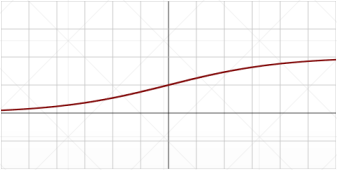
\includegraphics[width=0.5\textwidth]{sigmoid.png}
\end{figure}

\indent求导:
\begin{align*}
  \frac{d}{dx}\sigma(x) &=  \frac{d}{dx}(\frac{1}{1+e^{-x}})
  =\frac{e^{-x}}{(1+e^{-x})^2}\\
  &=\frac{e^{-x}+1-1}{(1+e^{-x})^2}
  =\sigma(1-\sigma)
\end{align*}
\begin{lstlisting}
  z = torch.linspace(-100,100,5)
  z   #tensor([-100.,  -50.,    0.,   50.,  100.])
  torch.sigmoid(z)   #tensor([0.00e+00, 1.92e-22, 5.00e-01, 1.00e+00, 1.00e+00])
\end{lstlisting}

\textbf{2. tanh}   常用于循环神经网络
$$f(x)=tanh(x)=\frac{e^x-e^{-x}}{e^x+e^{-x}}=2sigmoid(2x)-1~~~[-1,1]$$
\begin{figure}[!h]
  \centering
  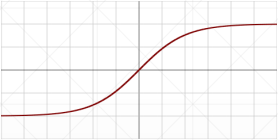
\includegraphics[width=0.5\textwidth]{tanh.png}
\end{figure}

求导:
\begin{align*}
\frac{d}{dx}tanh(x)=1-tanh^2(x)
\end{align*}
\begin{lstlisting}
  z = torch.linspace(-2, 2, 5)
  z   #tensor([-2., -1.,  0.,  1.,  2.])
  torch.tanh(z)   #tensor([-0.9640, -0.7616,  0.0000,  0.7616,  0.9640])
\end{lstlisting}


\textbf{2. ReLu}   Rectified Linear Unit 整形的线性单元 (最常用的激活函数)
\begin{equation}\nonumber
f(x)=
\begin{cases}
0& x<0\\
x& \geq 0
\end{cases}
\end{equation}求导:  \begin{equation}\nonumber
f(x)=
\begin{cases}
0& x<0\\
1& x\geq 0
\end{cases}
\end{equation}
\begin{figure}[!h]
  \centering
  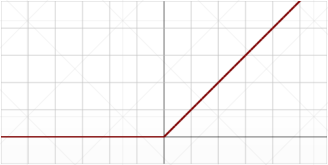
\includegraphics[width=0.5\textwidth]{relu.png}
\end{figure}
\begin{lstlisting}
  z = torch.linspace(-2, 2, 5)
  z   #tensor([-2., -1.,  0.,  1.,  2.])
  torch.relu(z)   #tensor([0., 0., 0., 1., 2.])
\end{lstlisting}

\subsection{Loss 损失函数的梯度}
\noindent典型的损失函数:
\begin{enumerate}
  \item Mean Squared Error(均方误差)
  \item Cross Entropy Loss(交叉熵损失 )
  \begin{itemize}
  \item 可用于二分类
  \item 可扩展为多分类
  \item 常与 softmax 函数搭配使用
\end{itemize}
\end{enumerate}




\noindent\textbf{1. Mean Squared Error(均方误差)}
\begin{itemize}
  \item $loss = \sum\big(y-(w*x+b)\big)^2$\\
  $loss = norm\big(y-(w*x+b)\big)^2$
  \item $\frac{\nabla loss}{\nabla \theta} = 2\sum \big(y-f_\theta(x)\big)*\frac{\nabla f_\theta(x)}{\nabla \theta}$
  \item Gradient API:\\
  \begin{lstlisting}
  1.torch.autograd.grad(loss, [w1, w2, ...])
    [w1 grad, w2 grad, ...]
  2.loss.backward()
    w1.grad
    w2.grad
    ...

  #Mean Square Error (MSE)
  x = torch.ones(1)
  y = torch.ones(1)
  w = torch.full([1], 2, requires_grad=True)
  mse = F.mse_loss(y,w*x)        #(y-w*x)
  mse   #tensor(1., grad_fn=<MeanBackward1>)
  #1.auto.grad  (requires_grad)
  torch.autograd.grad(mse, w)  #(tensor([2.]),)
  #2.backward
  mse = F.mse_loss(y,w*x)        #(y-w*x)
  mse.backward()
  w.grad   #tensor([2.])
\end{lstlisting}
\end{itemize}

\noindent\textbf{2. Cross Entropy Loss(交叉熵损失)}

\noindent\textbf{3. Softmax}
$$p_i=\frac{e^{a_i}}{\sum_{k=1}^{N}e^{a_k}}$$
\begin{figure}[!h]
  \centering
  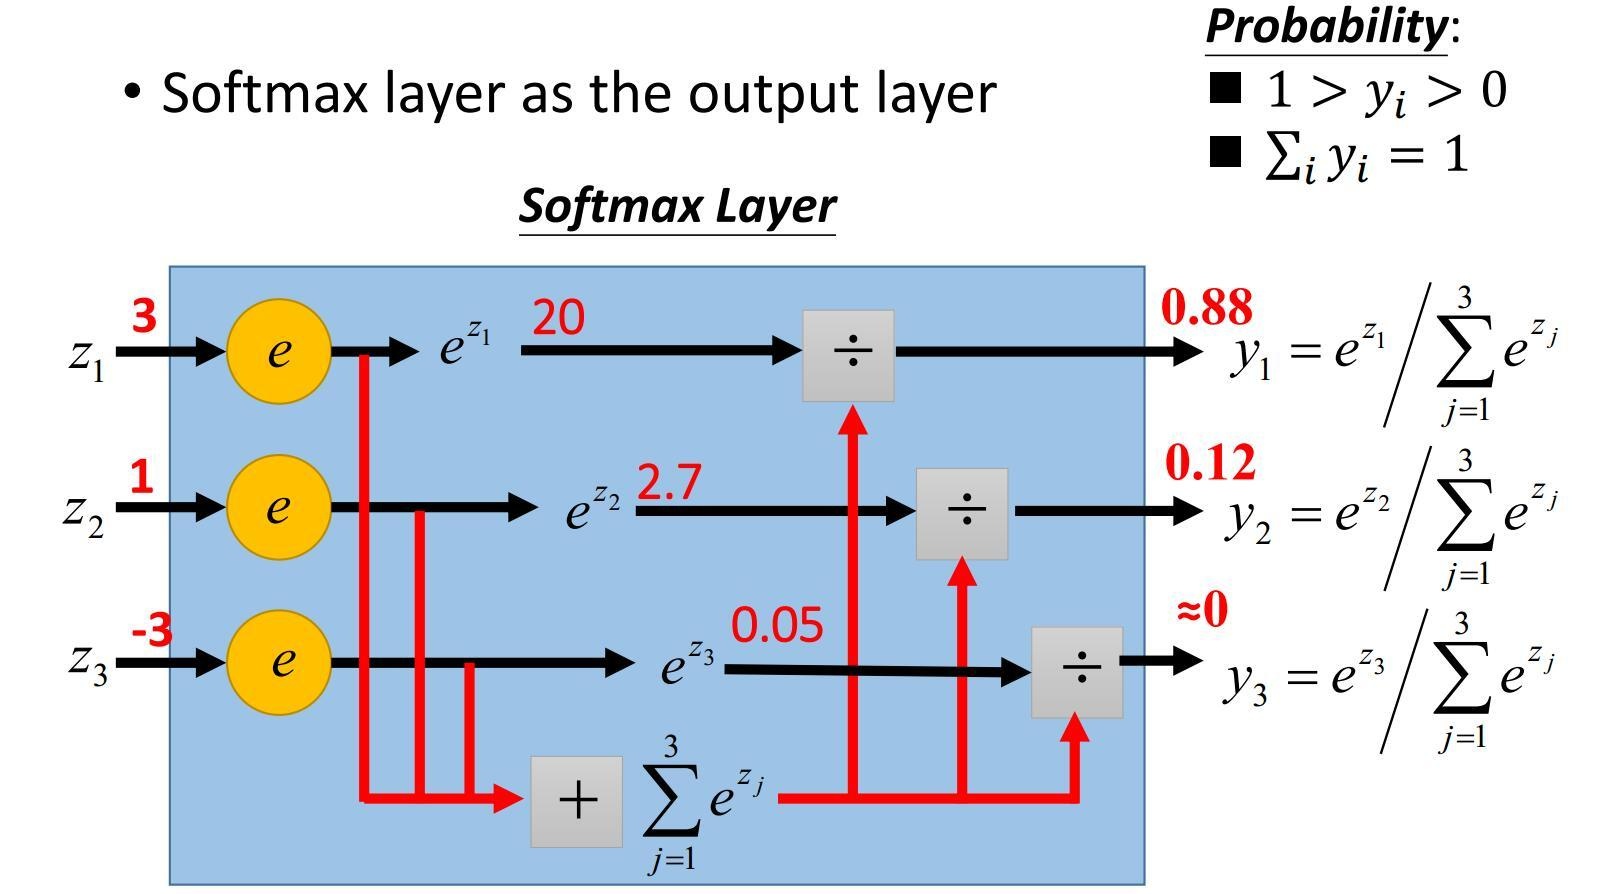
\includegraphics[width=1\textwidth]{softmax.jpg}
\end{figure}
\begin{enumerate}
  \item 转移成概率值
  \item 拉大值之间的差距
\end{enumerate}

\noindent\textbf{Softmax 求导:}
\begin{align*}
  &\frac{\partial p_i}{\partial a_j}=\frac{\partial\frac{e^{a_i}}{\sum_{k=1}^{N}e^{a_k}}}{\partial a_j}\\
  &f(x) = \frac{g(x)}{h(x)},~~~~~~~~~f'(x)=\frac{g'(x)h(x)-h'(x)g(x)}{h^2(x)}\\
  &g(x)=e^{a_i},~~~~~~~~~h(x)=\sum_{k=1}^{N}e^{a_k}
\end{align*}
\begin{align*}
  &i==j&&i\neq j\\
  \frac{\partial\frac{e^{a_i}}{\sum_{k=1}^{N}e^{a_k}}}{\partial a_j}&=\frac{e^{a_i} \sum_{k=1}^{N} e^{a_k}-e^{a_j}e^{a_i}}{\big(\sum_{k=1}^{N}e^{a_k}\big)^2}&\frac{\partial\frac{e^{a_i}}{\sum_{k=1}^{N}}}{\partial e^{a_j}}&=\frac{0-e^{a_j}e^{a_i}}{\big(\sum_{k=1}^{N}e^{a_k}\big)^2}\\
  &=\frac{e^{a_i}\big(\sum_{k=1}^{N}e^{a_k}-e^{a_j}\big)}{\big(\sum_{k=1}^{N}e^{a_k}\big)^2}&&=-\frac{e^{a_i}}{\sum_{k=1}^{N}e^{a_k}}\frac{e^{a^j}}{\sum_{k=1}^{N}e^{a_k}}\\
  &=p_i(1-p_j)&&=-p_ip_j
\end{align*}

\textbf{总结:}\\
\begin{equation}\nonumber
\frac{\partial p_i}{\partial a_j}=
\begin{cases}
p_i(1-p_i)& i==j\\
-p_ip_j& i\neq j
\end{cases}
\end{equation}

利用:
\begin{equation}\nonumber
\delta_{ij}=
\begin{cases}
1& i==j\\
0& i\neq j
\end{cases}
\end{equation}
\indent得到公式:
$$\frac{\partial p_i}{\partial a_j}=p_i(\delta_{ij}-p_j)$$
\begin{lstlisting}
  from torch.nn import functional as F
  a = torch.rand(3, requires_grad=True)
  p = F.softmax(a, dim=0)
  a   #tensor([0.4588, 0.0768, 0.0897], requires_grad=True)
  p   #tensor([0.4212, 0.2875, 0.2912], grad_fn=<SoftmaxBackward>)
  torch.autograd.grad(p[0], a, retain_graph=True)   #output scalar
      #(tensor([ 0.2438, -0.1211, -0.1227]),)
\end{lstlisting}


\newpage
\section{感知机梯度传播推导}
\subsection{单一输出感知机}
~\\
\begin{figure}[!h]
  \centering
  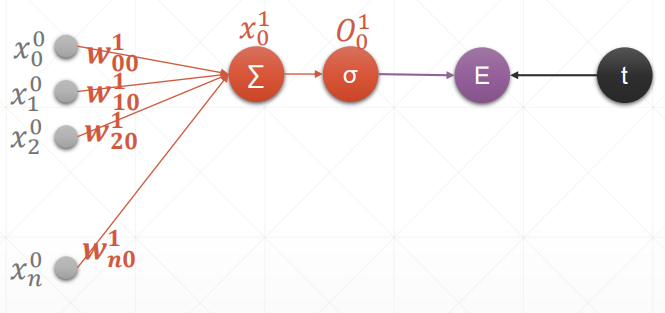
\includegraphics[width=0.67\textwidth]{perceptron1.png}
\end{figure}

\begin{align*}
  &E = \frac{1}{2}(O^1_0-t)^2\\
  &\frac{\partial E}{\partial w_{j0}}= (O^1_0-t)\frac{\partial O^1_0}{\partial w_{j0}}=(O^1_0-t)\frac{\partial \sigma(x_0^1)}{\partial w_{j0}}\\
  &\frac{\partial E}{\partial w_{j0}}=(O^1_0-t)\sigma(x^1_0)(1-\sigma(x^1_0))\frac{\partial x^1_0}{\partial w_{j0}}\\
  &\frac{\partial E}{\partial w_{j0}}=(O^1_0-t)\sigma(x^1_0)(1-\sigma(x^1_0))x^0_j\\
  &\textcolor{red}{\frac{\partial E}{\partial w_{j0}}=(O^1_0-t)O^1_0(1-O^1_0)x^0_j}
\end{align*}
~\\
\begin{lstlisting}
x = torch.randn(1, 10)
w = torch.randn(1, 10, requires_grad=True)
o = torch.sigmoid(x@w.t())
o.shape     #torch.Size([1, 1])
loss = F.mse_loss(torch.ones(1, 1), o)
loss.shape     #torch.Size([])  scalar
loss.backward()
w.grad   #tensor([[ 2.1023e-04, -4.6425e-04,  2.1561e-04,...]])
\end{lstlisting}

\newpage
\subsection{多输出感知机}
~\\
\begin{figure}[!h]
  \centering
  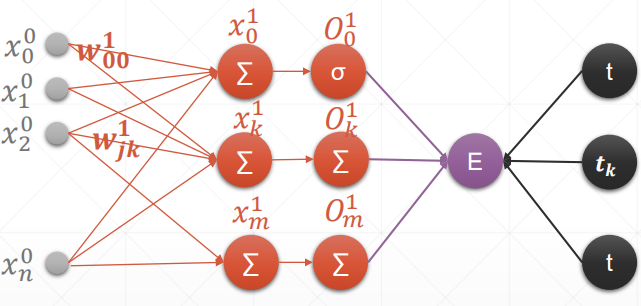
\includegraphics[width=0.8\textwidth]{perceptron2.png}
\end{figure}

\begin{align*}
  &E = \frac{1}{2}\sum_{i=0}^{m}(O^1_i-t)^2\\
  &\frac{\partial E}{\partial w_{jk}}= (O^1_k-t_k)\frac{\partial O^1_k}{\partial w_{jk}}=(O^1_k-t_k)\frac{\partial \sigma(x_k^1)}{\partial w_{jk}}\\
  &\frac{\partial E}{\partial w_{jk}}=(O^1_k-t_k)\sigma(x^1_k)(1-\sigma(x^1_k))\frac{\partial x^1_k}{\partial w_{jk}}\\
  &\frac{\partial E}{\partial w_{jk}}=(O^1_k-t_k)\sigma(x^1_k)(1-\sigma(x^1_k))x^0_j\\
  &\textcolor{red}{\frac{\partial E}{\partial w_{jk}}=(O^1_k-t_k)O^1_k(1-O^1_k)x^0_j}
\end{align*}
~\\
\begin{lstlisting}
x = torch.rand(1, 10)
w = torch.rand(2, 10, requires_grad=True)
o = torch.sigmoid(x@w.t())
o.shape     #torch.Size([1, 2])
loss = F.mse_loss(torch.ones(1,2), o)
loss      #tensor(0.0158, grad_fn=<MeanBackward1>)
loss.backward()
w.grad.shape     #torch.Size([2, 10])
\end{lstlisting}




\subsection{链式法则}
\subsubsection{求导法则}
\begin{figure}[!h]
  \centering
  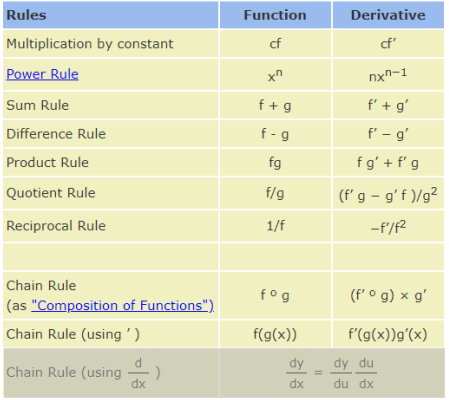
\includegraphics[width=0.86\textwidth]{chain.png}
\end{figure}

\subsubsection{链式法则公式}

$$\frac{\partial y}{\partial x} = \frac{\partial y}{\partial u}\frac{\partial u}{\partial x}$$

\begin{lstlisting}
x = torch.tensor(1.)
w1 = torch.tensor(2., requires_grad=True)
b1 = torch.tensor(1.)
w2 = torch.tensor(2., requires_grad=True)
b2 = torch.tensor(1.)
y1 = x*w1 + b1
y2 = y1*w2 + b2
dy2_dy1 = torch.autograd.grad(y2, y1, retain_graph=True)[0]
dy1_dw1 = torch.autograd.grad(y1, w1, retain_graph=True)[0]
dy2_dw1 = torch.autograd.grad(y2, w1, retain_graph=True)[0]
dy2_dw1, dy2_dy1, dy1_dw1     #tensor(2.) tensor(2.) tensor(1.)
\end{lstlisting}


\subsection{MLP 反向传播推导}
~\\
\begin{figure}[!h]
  \centering
  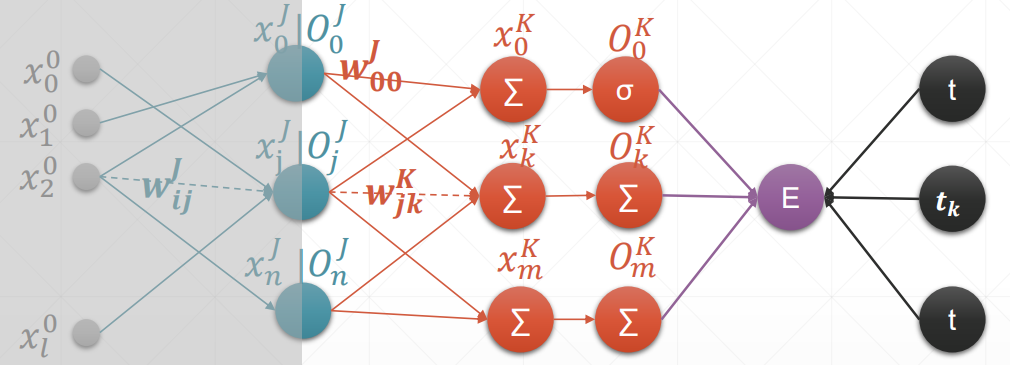
\includegraphics[width=0.86\textwidth]{MLP.png}
\end{figure}

\begin{align*}
  &\text{那么第K层的权值偏微分可知:}\\
  &\frac{\partial E}{\partial w^K_{jk}} = (O^K_k - t_k)O^K_k(1-O^K_k)O^J_j\\
  \text{令}~~~&\textcolor{red}{\delta^K_k = (O^K_k - t_k)O^K_k(1-O^K_k)}\\
  &\textcolor{red}{\frac{\partial E}{\partial w^K_{jk}} = \delta^K_k O^J_j}\\
  &\text{那么再求第J层的权值偏微分:}\\
  &\frac{\partial E}{\partial w_{ij}} = \frac{\partial }{\partial w_{ij}}\frac{1}{2}\sum_{k\in K}(O_k-t_k)^2\\
  &\frac{\partial E}{\partial w_{ij}} = \sum_{k \in K}(O_k - t_k)\frac{\partial }{w_{ij}}O_k=\sum_{k \in K}(O_k - t_k)\frac{\partial }{w_{ij}}\sigma(x_k)\\
  &\frac{\partial E}{\partial w_{ij}}=\sum_{k \in K}(O_k - t_k)\sigma(x_k)(1-\sigma(x_k))\frac{\partial x_k}{\partial w_{ij}}\\&~~~~~~~~~=\sum_{k \in K}(O_k - t_k)\sigma(x_k)(1-\sigma(x_k))\frac{\partial x_k}{\partial O_j}\cdot \frac{\partial O_j}{\partial w_{ij}}\\
  &~~~~~~~~~=\sum_{k \in K}(O_k - t_k)O_k(1-O_k)w^K_{jk} \frac{\partial O_j}{\partial w_{ij}}=\frac{\partial O_j}{\partial w_{ij}} \sum_{k \in K}(O_k - t_k)O_k(1-O_k)w^K_{jk}\\
  &~~~~~~~~~=O_j(1-O_j)\frac{\partial x_j}{\partial w_{ij}}\sum_{k \in K}(O_k - t_k)O_k(1-O_k)w^K_{jk}\\
  &~~~~~~~~~=O_j(1-O_j)O_i\sum_{k \in K}(O_k - t_k)O_k(1-O_k)w^K_{jk}\\
  \text{令}~~~&\textcolor{red}{\delta^J_j= O_j(1-O_j)\sum_{k\in K}\delta_kw_{jk}}\\
  &\textcolor{red}{\frac{\partial E}{\partial w_{ij}}=O^I_i\delta_j}
\end{align*}
\textcolor{red}{总结}:
\textbf{\begin{align*}
  &\text{对于一个输出层的节点}~~k \in K\\
  &~~~~~~~~~~~~~~~~~~~~~~~~~~~~~~~~~~~~~~~~~~~~~\frac{\partial E}{\partial w_{jk}}=O_j\delta_k\\
  &\text{这里,}\\
  &~~~~~~~~~~~~~~~~~~~~~~~~~~~~~~~~~~~\delta_k=O_k(1-O_k)(O_k-t_k)\\
  &\text{对于一个隐藏层的节点}~~j \in J\\
  &~~~~~~~~~~~~~~~~~~~~~~~~~~~~~~~~~~~~~~~~~~~~~\frac{\partial E}{\partial w_{ij}}=O_i\delta_j\\
  &\text{这里,}\\
  &~~~~~~~~~~~~~~~~~~~~~~~~~~~~~~~~~~~\delta_j=O_j(1-O_j)\sum_{k\in K}\delta_k w_{jk}
\end{align*}}
~\\
~\\

\begin{figure}[!h]
  \centering
  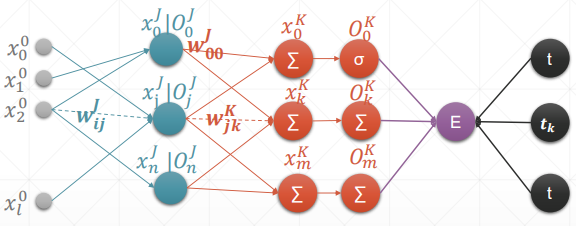
\includegraphics[width=0.86\textwidth]{MLP2.png}
\end{figure}

正向传播:$$O^J~~-->~~O^K~~-->~~E$$

反向传播:$$\delta^K~~-->~~\frac{\partial E}{\partial w^K}~~-->~~\delta^J~~-->~~\frac{\partial E}{\partial w^J}~~-->~~\delta^L~~-->~~\frac{\partial E}{\partial w^L}$$

\newpage
\subsection{2D 函数优化实例}
$$f(x,y)=(x^2 + y - 11)^2+(x+y^2-7)^2$$
\begin{figure}[!h]
  \centering
  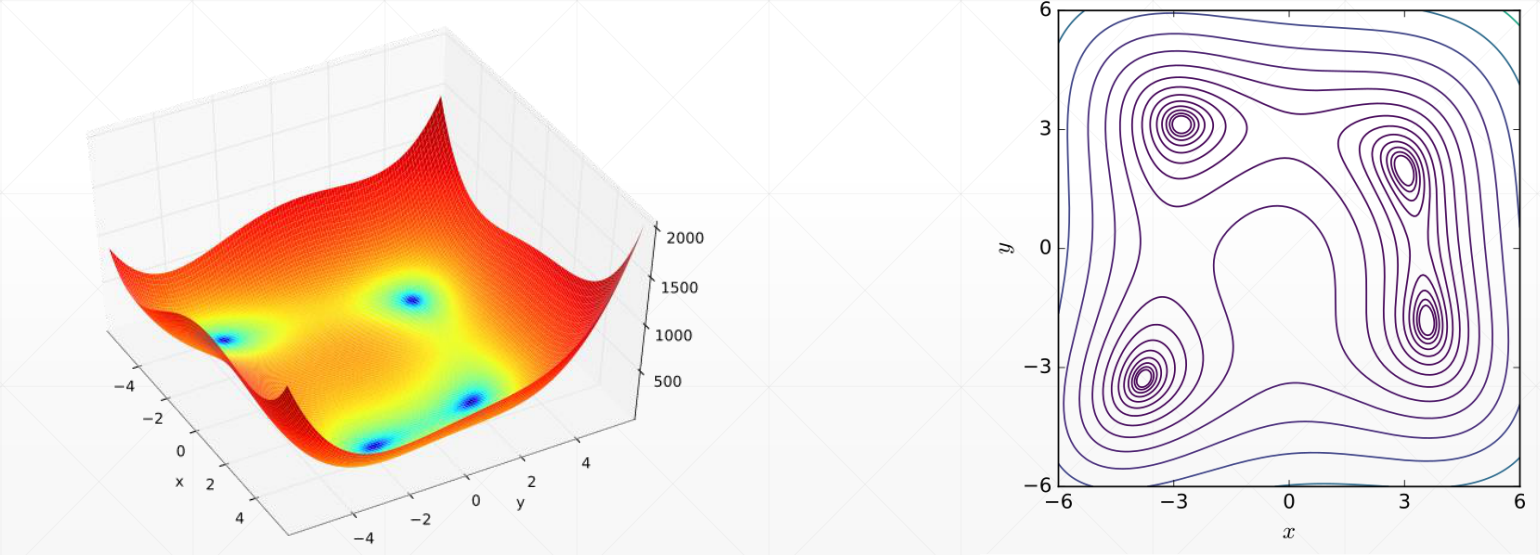
\includegraphics[width=1\textwidth]{plt.png}
\end{figure}

\textbf{minma:}
\begin{itemize}
  \item $f(3, 2)=0$
  \item $f(-2.805118, 3.131312)=0$
  \item $f(-3.779310, -3.283186)=0$
  \item $f(3.584428, -1.848126)=0$
\end{itemize}

\textbf{绘图 3d}
\begin{lstlisting}
import numpy as np
import matplotlib.pyplot as plt

def himmelblau(x):
    return (x[0]**2+x[1]-11)**2+(x[0]+x[1]**2-7)**2

x = np.arange(-6, 6, 0.1)
y = np.arange(-6, 6, 0.1)
print ('x,y range:', x.shape, y.shape)
X, Y = np.meshgrid(x, y)
print ('X,Y range:', X.shape, Y.shape)
Z = himmelblau([X,Y])

fig = plt.figure('himmelblau')
ax = fig.gca(projection='3d')
ax.plot_surface(X, Y, Z)
#ax.view_init(60, -30)
ax.set_xlabel('x')
ax.set_ylabel('y')
plt.show()
\end{lstlisting}
\begin{figure}[!h]
  \centering
  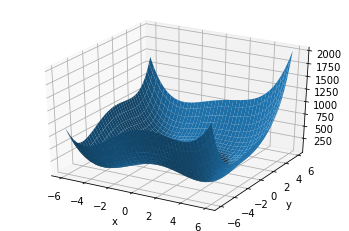
\includegraphics[width=0.78\textwidth]{hemm.png}
\end{figure}

\textbf{优化}
\begin{lstlisting}
import torch
x = torch.tensor([0., 0.], requires_grad=True)
optimizer = torch.optim.Adam([x], lr=1e-3)  # '建立梯度更新式 x:=x-grad\_x'
for step in range(20000):
    pred = himmelblau(x)  #'得到预测值'
    optimizer.zero_grad()   #'清零梯度值'
    pred.backward()     #'得到 x 的梯度'
    optimizer.step()     #'更新 x 梯度'

    if step % 2000 == 0:
        print ('step {}: x = {}, f(x) = {}'.format(step, x.tolist(), pred.item()))
\end{lstlisting}







\newpage
\section{多层感知机与分类器}
\subsection{逻辑回归}
\begin{enumerate}
  \item 对于逻辑回归我们不能直接最大化 accuracy。
  \begin{itemize}
    \item acc.= $\frac{I(pred_i==y_i)}{len(Y)}$
    \item grad 出现等于零的情况。
    \item grad 不连续。
  \end{itemize}
  \item 为什么叫 regression。
  \begin{itemize}
    \item MSE$-->$regression.
    \item cross entropy$-->$classification.
  \end{itemize}
  \item 多类:
  \begin{itemize}
    \item 实现多个二分类器。
    \item softmax。
  \end{itemize}
\end{enumerate}


~\\
~\\~\\~\\
\subsection{交叉熵}
\subsubsection{Entropy}
\begin{enumerate}
  \item uncertain 不确定度
  \item measure of surprise 惊喜程度
  \item higher entropy = less info \\
  $$entropy = -\sum_{i}P(i)logP(i)$$
\end{enumerate}

\subsubsection{Cross Entropy}
$$H(p,q) = \sum p(x)log q(x)$$
$$H(p,q) = H(p)+D_{KL}(p|q)$$
$$p=q, ~~~Cross~entropy=entropy$$
$$H(P,Q)=-(ylogp+(1-y)log(1-p))$$


\noindent \textbf{对于分类为什么不用MSE:}
\begin{enumerate}
  \item sigmoid+MSE(梯度弥散)。
  \item 收敛非常慢。
  \item 但是有时可以试试MSE, 求导简单。
\end{enumerate}

\noindent \textbf{小结:}
$$logit-->softmax-->cross~entropy$$
\indent 一般不建议自己单独使用 softmax 与 cross entropy。 使用 pytorch 组合的框架。
\begin{lstlisting}
import torch
from torch.nn import functional as F
x = torch.randn(1,784)
w = torch.randn(10,784)
logits = x@w.t()
pred = F.softmax(logits, dim=1)
pred_log = torch.log(pred)
F.nll_loss(pred_log, torch.tensor([1]))   #F.cross_entropy=F.softmax+log+F.nll_loss
F.cross_entropy(logits, torch.tensor([1]))
\end{lstlisting}


\newpage
\subsection{多分类实战-Mnist}
\begin{figure}[!h]
  \centering
  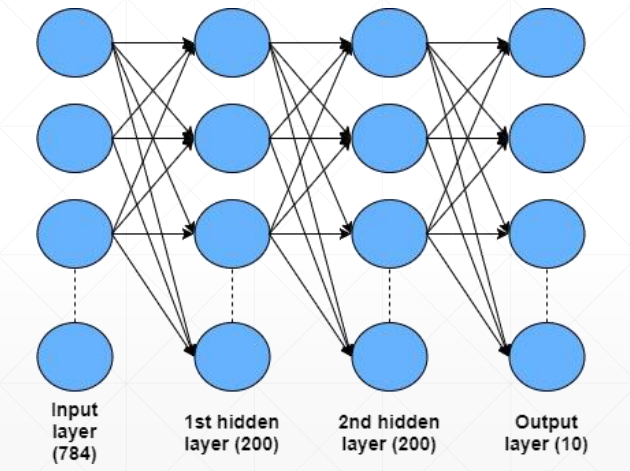
\includegraphics[width=0.8\textwidth]{multipleC.png}
\end{figure}

\textbf{建立网络:}
\begin{lstlisting}
  w1, b1 = torch.randn(200, 784, requires_grad=True), torch.zeros(200, requires_grad=True)
  w2, b2 = torch.randn(200, 200, requires_grad=True), torch.zeros(200, requires_grad=True)
  w3, b3 = torch.randn(10, 200, requires_grad=True), torch.zeros(10, requires_grad=True)

  '\#向前传播'
  def forward(x):
      x = x@w1.t()+b1
      x = F.relu(x)
      x = x@w2.t()+b2
      x = F.relu(x)
      x = x@w3.t()+b3
      x = F.relu(x)
      return x
\end{lstlisting}

\textbf{训练:}
\begin{lstlisting}
optimizer = optim.SGD([w1, b1, w2, b2, w3, b3], lr=learning_rate)
criteon = nn.CrossEntropyLoss()

for epoch in range(epochs):

    '\#训练'
    for batch_idx, (data, target) in enumerate(train_loader):
        data = data.reshape(-1, 28*28)     #torch.Size([200, 784])

        logits = forward(data)    #torch.Size([200, 10])
        loss = criteon(logits, target)

        optimizer.zero_grad()     '\#梯度清零'
        loss.backward()     '\#反向回传'
#        print(w1.grad.norm(), w2.grad.norm())
        optimizer.step()    '\#更新梯度值'
\end{lstlisting}

\textcolor{red}{通过打印 weight.grad.norm(),得知常常陷入局部极小值。解决这个问题可以利用何凯明的初始化方法。}
\begin{lstlisting}
torch.nn.init.kaiming_normal_(w1)
torch.nn.init.kaiming_normal_(w2)
torch.nn.init.kaiming_normal_(w3)
\end{lstlisting}
~\\~\\~\\~\\



\subsection{全连接层}
在上节中, 我们未用 PyTorch 封装的 API 去建立神经网络,这节来使用 PyTorch 封装的 API。
\begin{enumerate}
  \item 继承 nn.module 类
  \item 用 \_\_init\_\_ 来初始化
  \item 应用向前传播
\end{enumerate}
  \begin{lstlisting}
  class MLP(nn.Module):

    def __init__(self):
        super(MLP, self).__init__()

        self.model = nn.Sequential(
            nn.Linear(784, 200),
            nn.ReLU(inplace=True),
            nn.Linear(200, 200),
            nn.ReLU(inplace=True),
            nn.Linear(200, 10),
            nn.ReLU(inplace=True),
        )

    def forward(self, x):
        x = self.model(x)
        return x
  \end{lstlisting}

\noindent\textbf{PyTorch 两种风格的API}
  \begin{enumerate}
    \item class-style API (nn.***)
    \item function-style API (F.***)
  \end{enumerate}

\textcolor{red}{{没有遇到上节遇到的初始化问题, 参数未暴露给用户, 拥有自己的初始化体系,一般来说够用,否则自己必须编写相应的初始化代码。}}


~\\~\\~\\~\\



\subsection{激活函数与GPU加速}
\subsubsection{常用激活函数}
\begin{enumerate}
  \item Sigmoid
  \item ReLu
  \item tanh
  \item Leaky ReLu
  \item SELU
  \item softplus
\end{enumerate}
\subsubsection{一键部署 GPU 加速}
\begin{lstlisting}
device = torch.device('cuda')
net = MLP().to(device)
optimizer = optim.SGD(net.parameters(), lr=learning_rate)
criteon = nn.CrossEntropyLoss().to(device)

time1 = time.time()
for epoch in range(epochs):

    for batch_idx, (data, target) in enumerate(train_loader):
        data = data.view(-1, 28*28)
        data, target = data.to(device), target.cuda()

        logits = net(data)
        loss = criteon(logits, target)

        optimizer.zero_grad()
        loss.backward()
        optimizer.step()
\end{lstlisting}
~\\~\\~\\~\\


\subsection{测试与可视化}
\subsubsection{测试}
\textbf{神经网络的表达能力非常强,容易过拟合,所以要测试。不能单一观测  Loss 的大小判断模型的好坏,还要观测测试集的准确度,确保模型的泛化能力。}
\begin{lstlisting}
    test_loss = 0
    correct = 0
    for data, target in test_loader:
        data = data.view(-1, 28 * 28)
        data, target = data.to(device), target.cuda()
        logits = net(data)
        test_loss += criteon(logits, target).item()

        pred = logits.argmax(1)
        correct += pred.eq(target.data).sum()

    test_loss /= len(test_loader.dataset)
\end{lstlisting}

\subsubsection{可视化-Visdom}
通过pip install visdom等方式成功安装完之后,开启服务
\begin{lstlisting}
  python -m visdom.server
\end{lstlisting}

\textcolor{red}{出现了Mnist图片 viz.images() 全黑故障,估计是由于样本标准化引起的。}




\newpage
\section{深度学习的其他技巧}
\subsection{过拟合与欠拟合}
\subsubsection{欠拟合}
\begin{figure}[!h]
  \centering
  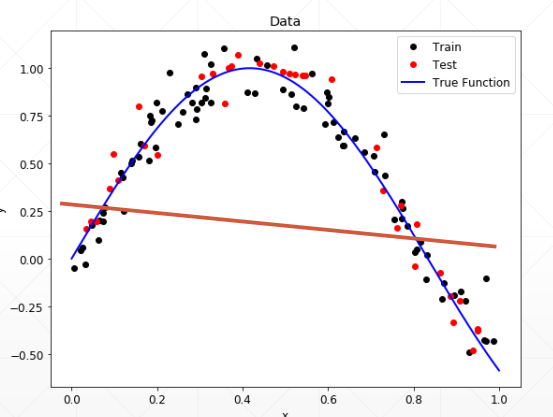
\includegraphics[width=0.6\textwidth]{underfitting.png}
\end{figure}

\textbf{模型简单,表达能力不够,导致欠拟合。}

\subsubsection{过拟合}
\begin{figure}[!h]
  \centering
  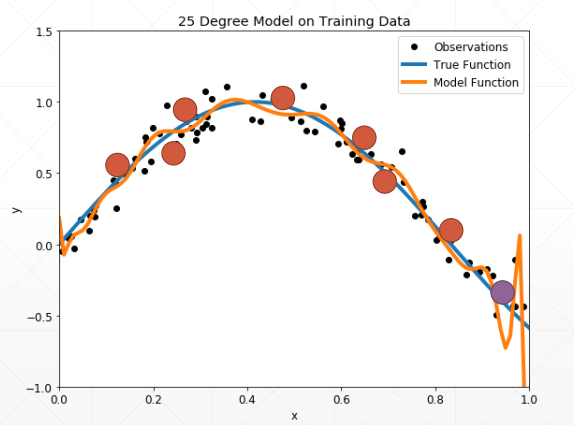
\includegraphics[width=0.6\textwidth]{overfitting.png}
\end{figure}

\textbf{现实生活中更多地是过拟合,模型表达能力太强,数据量太少导致的。}

\textcolor{red}{那如何检测过拟合状况,当发生了过拟合如何减少过拟合,是要着重考虑和解决的问题。}

\textcolor{red}{检测过拟合-交叉验证}

\textcolor{red}{防止过拟合-正则化}

\newpage


\subsection{交叉验证}
\subsubsection{数据划分}
过拟合是模型学习过程中非常重要的一个问题。那么如何检测过拟合也是非常重要的。通过在数据集划分进行训练测试,寻找在过拟合之前的最优参数。
\begin{figure}[!h]
  \centering
  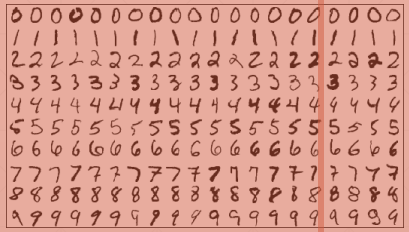
\includegraphics[width=0.8\textwidth]{splitting.png}
\end{figure}

\textbf{事实上将数据划分成训练集, 验证集, 测试集。}
\begin{figure}[!h]
  \centering
  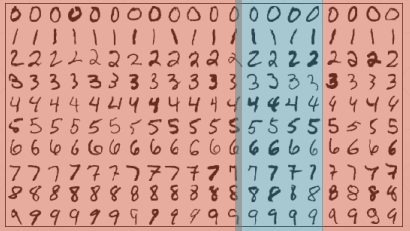
\includegraphics[width=0.8\textwidth]{TVT.png}
\end{figure}

\textcolor{red}{将数据划分成三类,客户用保密的测试集来测试模型效果,防止作弊。}
\begin{lstlisting}
train_db = datasets.MNIST('../data', train=True, download=True,
                   transform=transforms.Compose([
                       transforms.ToTensor(),
                       transforms.Normalize((0.1307,), (0.3081,))
                   ]))
train_loader = torch.utils.data.DataLoader(
    train_db,
    batch_size=batch_size, shuffle=True)

test_db = datasets.MNIST('../data', train=False, transform=transforms.Compose([
    transforms.ToTensor(),
    transforms.Normalize((0.1307,), (0.3081,))
]))
test_loader = torch.utils.data.DataLoader(test_db,
    batch_size=batch_size, shuffle=True)


print('train:', len(train_db), 'test:', len(test_db))
train_db, val_db = torch.utils.data.random_split(train_db, [50000, 10000])
print('db1:', len(train_db), 'db2:', len(val_db))
train_loader = torch.utils.data.DataLoader(
    train_db,
    batch_size=batch_size, shuffle=True)
val_loader = torch.utils.data.DataLoader(
    val_db,
    batch_size=batch_size, shuffle=True)
\end{lstlisting}
~\\~\\~\\
\subsubsection{K-fold交叉验证}
\begin{figure}[!h]
  \centering
  
\includegraphics[width=1\textwidth]{Kfold.png}
\end{figure}

\textbf{将训练集划分成十份,每次将其中九份用于训练,一份用于验证,选择较好的时间戳权值参数。}



\subsection{正则化}
\subsubsection{奥卡姆剃刀原理}
\textbf{能使用简单模型参数量解决的模型问题不要使用复杂模型的参数量。}

\textbf{More things should not be used than are necessary}

\subsubsection{防止过拟合的方法}
\begin{enumerate}
  \item 数据扩充
  \item 限制模型的复杂度
  \begin{itemize}
    \item 浅层网络
    \item 添加正则化项
  \end{itemize}
  \item Dropout
  \item Data argument(数据增强)
  \item Early Stop
\end{enumerate}



\subsubsection{正则化}
\textbf{Regularization == Weight Decay}
\begin{enumerate}
  \item L1范数
  $$J(\theta)=-\frac{1}{m}\sum_{i=1}^{m}\big[y_ilog\hat{y_i}+(1-y_i)log(1-y_i)+\lambda\sum_{i=1}^{n}|\theta|\big]$$
  \begin{lstlisting}
    regularizatin_loss = 0
    for param in model.parameters():
        regularization_loss += torch.sum(torch.abs(param))

    classify_loss = criteon(logits, target)
    loss = classify_loss + 0.01 + regularization_loss

    optimizer.zero_grad()
    loss.backward()
    optimizer.step()
  \end{lstlisting}
  \item L2范数
  $$J(\theta)=-\frac{1}{m}\sum_{i=1}^{m}\big[y_ilog\hat{y_i}+(1-y_i)log(1-y_i)+\frac{1}{2}\lambda||W||^2\big]$$
  \begin{lstlisting}
  net = MLP().to(device)
  optimizer = optim.SGD(net.parameters(), lr=learning_rate, weight_decay=0.01)
  criteon = nn.CrossEntropyLoss().to(device)
  \end{lstlisting}
\end{enumerate}



\subsection{动量与学习率衰减}
\subsubsection{动量}
\textbf{momentum 动量也称惯性}
\begin{align*}
  &&w^{k+1}=w^{k}-\alpha\nabla f(w^k)\\
  &&\\
  &&z^{k+1}=\beta z^k + \nabla f(w^k)\\
  &&w^{k+1}=w^k-\alpha z^{k+1}
\end{align*}
加入动量的迭代式,实际上就是当前的梯度方向加上上一次的惯性的方向。尽快收敛,并且大概率的跳出局部极小值。

\begin{enumerate}
  \item 没加动量的例子\\
\begin{figure}[!h]
  \centering
  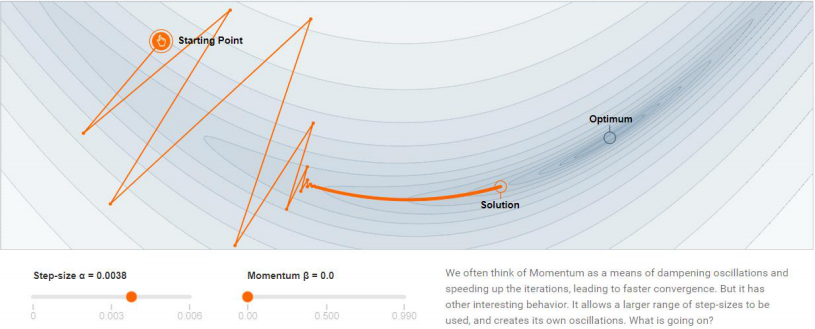
\includegraphics[width=1\textwidth]{NoMomentum.png}
\end{figure}\\
    梯度更新刁钻,迭代效率低,容易陷入局部极小。\\
    ~\\
  \item 引入动量的例子\\
  \begin{figure}[!h]
  \centering
  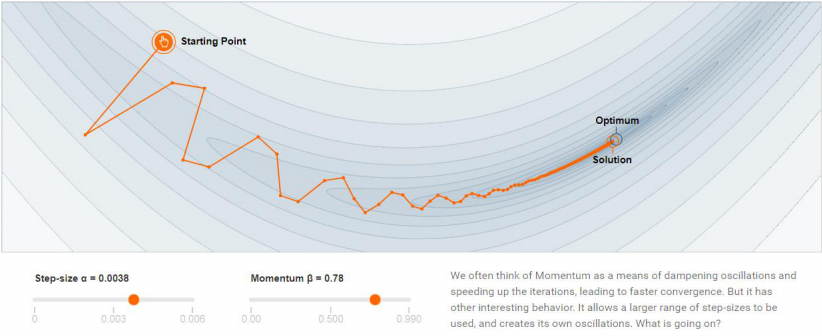
\includegraphics[width=1\textwidth]{WithMomentum.png}
\end{figure}\\
    梯度更新效率高,越过了局部极小,步入全局最小。
\begin{lstlisting}
  optimizer = torch.optim.SGD(model.parameters(), args.lr,
                                momentum=args.momentum,
                                weight_decay=args.weight_decay)
\end{lstlisting}
\textcolor{red}{~~~~~~PyTorch 中 Adam 优化器已经内置了 momentum 机制,所以不需要变量维护;但是 SGD 却没有。}
\end{enumerate}



\subsubsection{学习率衰减}
\textbf{learning rate decay}
\begin{figure}[!h]
  \centering
  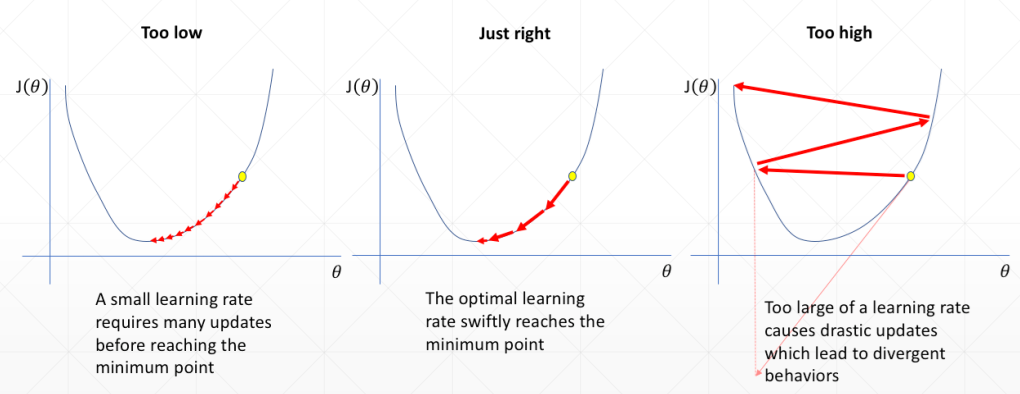
\includegraphics[width=0.85\textwidth]{LearningRate.png}
\end{figure}

\noindent Learning Rate 设置过大,导致摇摆,得不到较好的效果。\\
Learning Rate 设置过小,更新迭代次数过多。

~\\
~\\
\begin{figure}[!h]
  \centering
  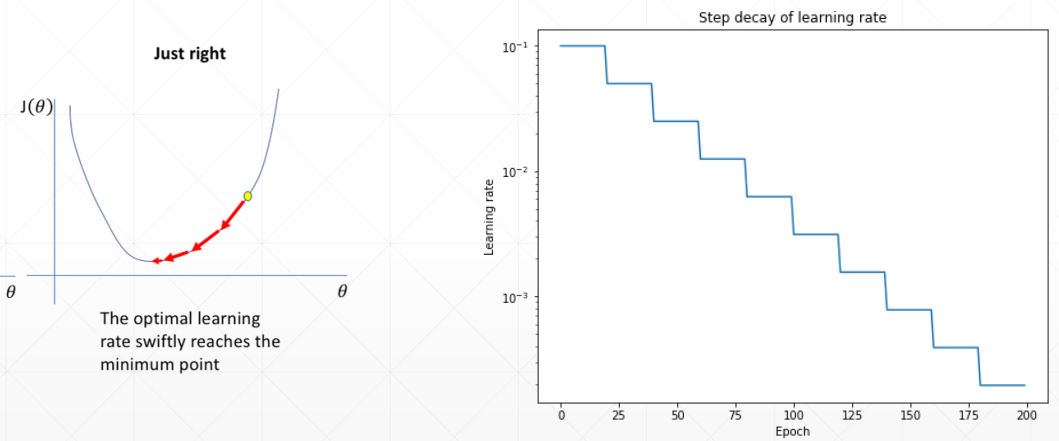
\includegraphics[width=0.85\textwidth]{LRate.png}
\end{figure}
 学习率衰减,刚开始选择大一点的学习率,也不会较大影响,前期还能较快更新。

 ~\\
 \textbf{PyTorch 设置学习率衰减}
 \begin{enumerate}
   \item 方法一     遇平原衰减
   \begin{lstlisting}
  optimizer = torch.optim.SGD(model.parameters(), args.lr,
                                momentum=args.momentum,
                                weight_decay=args.weight_decay)
  schedule = ReduceLROnPlateau(optimizer, 'min')     #'学习率衰减监听'

  for epoch in xrange(args.start_opech, args.epochs):
      train(train_loader, model, criterion, optimizer, epoch)
      result_avg, loss_val = validate(val_model, criterion, epoch)
      schedule.step(loss_val)
\end{lstlisting}
   \item 方法二     定时衰减
\begin{lstlisting}
  #Assuming optimizer uses lr = 0.05 for all groups
  #lr = 0.05           if epoch < 30
  #lr = 0.005          if 30 <= epoch <= 60
  #lr = 0.0005         if 60 <= epoch <= 90
  # ...
  scheduler = StepLR(optimizer, step_size=30, gamma=0.1)
  for epoch in range(100)
  schedule.step()
  train(...)
  validate(...)
\end{lstlisting}
 \end{enumerate}


\subsection{提前停止更新与Dropout}
\subsubsection{提前停止更新}
提前停止更新是为了模型学习过拟合。

\begin{figure}[!h]
  \centering
  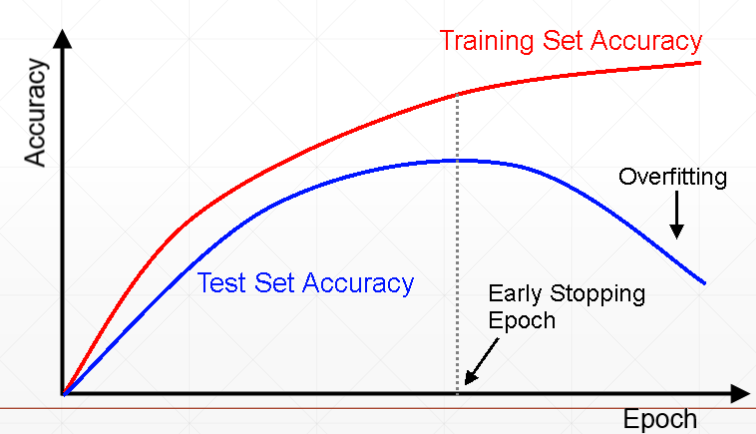
\includegraphics[width=0.6\textwidth]{EarlyStop.png}
\end{figure}

\subsubsection{Dropout}
dropout 也是防止过拟合常用的小技巧。
\begin{enumerate}
  \item Learning less to learn better
  \item Each connection has �$\rho$= 0, 1 to lose
\begin{figure}[!h]
  \centering
  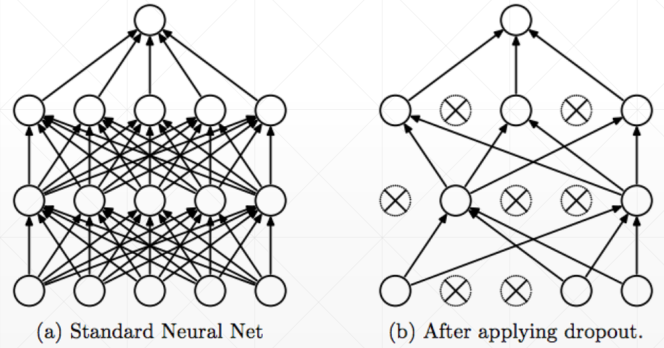
\includegraphics[width=0.76\textwidth]{dropout1.png}
\end{figure}
\end{enumerate}
\begin{lstlisting}
  net_dropped = torch.nn.Sequential(
      torch.nn.Linear(784, 200),
      torch.nn.Dropout(0.5),    #dropout 50% of the neuron
      torch.nn.ReLU(),
      torch.nn.Linear(200, 200),
      torch.nn.Dropout(0.5),    #dropout 50% of the neuron
      torch.nn.ReLU(),
      torch.nn.Linear(200, 10)
  )
\end{lstlisting}

\textbf{在训练时,我们把部分连接断掉;但是在测试或者验证时,必须把状态切换回来。}
\begin{lstlisting}
  for epoch for range(epochs):

      # train
      net_dropped.train()
      for batch_idx, (data, target) in enumerate(train_loader):
          ...

      net_dropped.eval()
      test_loss = 0
      correct = 0
      for data, target in test_loader:
          ...
\end{lstlisting}


\newpage
\section{卷积神经网络}
\subsection{卷积}
\begin{figure}[!h]
  \centering
  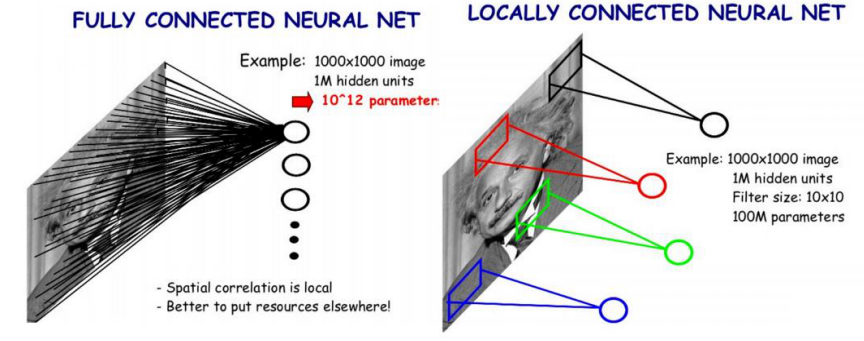
\includegraphics[width=0.9\textwidth]{FullLocal.png}
\end{figure}
卷积实则是一种特征映射,解决了在线性全连接层下的参数维度过大的问题。同时卷积也来源于人类视觉局部性的感受区域。\textbf{参数共享}是卷积神经网络的一个重要特征,也极大地减少了参数维度。
\begin{figure}[!h]
  \centering
  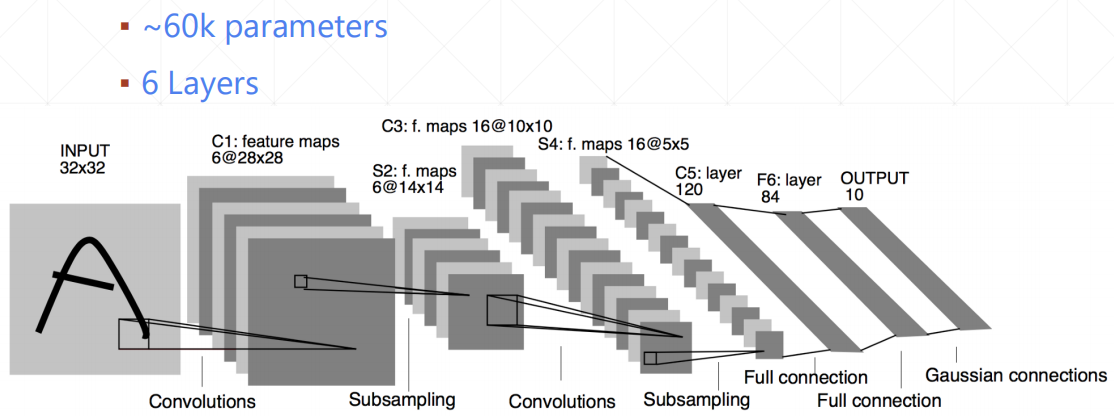
\includegraphics[width=0.9\textwidth]{CNN.png}
\end{figure}

卷积一次来源于信号处理上两个函数之间的卷积运算,操作可视化后类似。
\begin{figure}[!h]
  \centering
  \includegraphics[width=0.6\textwidth]{conv.png}
\end{figure}


\subsection{卷积神经网络}
\subsubsection{notation}
\begin{figure}[!h]
  \centering
  \includegraphics[width=0.5\textwidth]{notation.png}
\end{figure}
\begin{enumerate}
  \item Input\_channels
  \item Kernel\_channels: 2ch
  \item Kernel\_size
  \item Stride  ~~步幅。
  \item Padding  ~~填充。
\end{enumerate}

\subsubsection{Multi-Kernel}
\begin{figure}[!h]
  \centering
  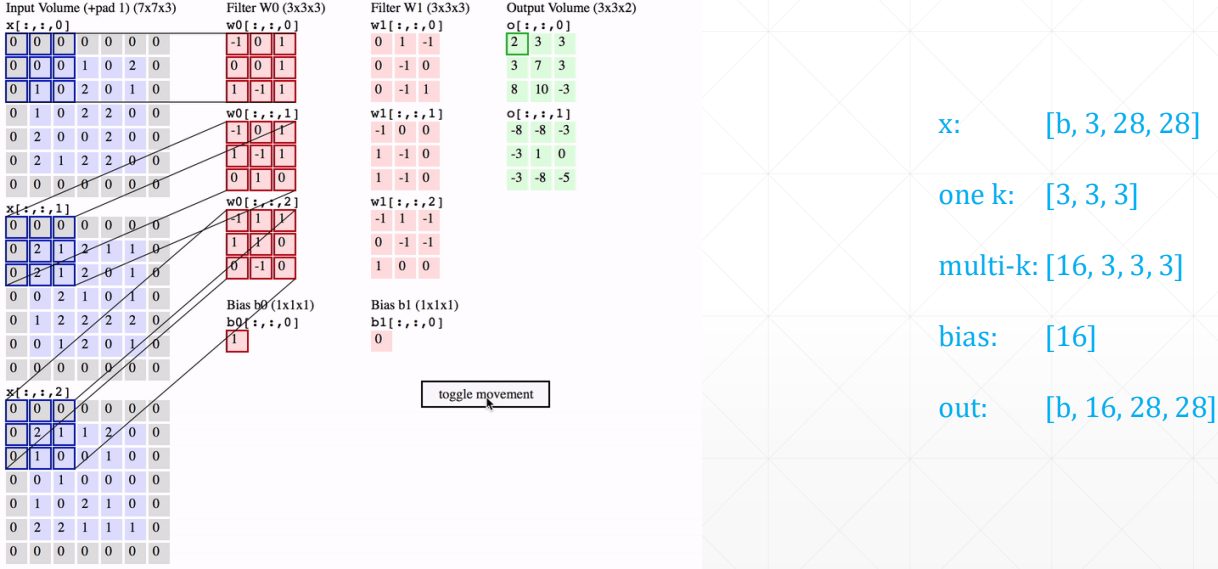
\includegraphics[width=0.9\textwidth]{multiKernel.png}
\end{figure}

\subsubsection{LeNet-5}
\begin{figure}[!h]
  \centering
  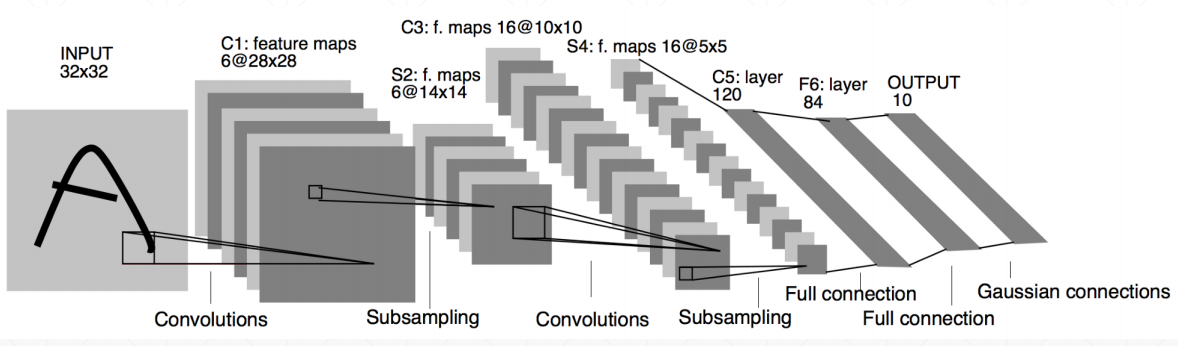
\includegraphics[width=1\textwidth]{LeNet.png}
\end{figure}

\subsubsection{卷积层的作用效果}
\begin{figure}[!h]
  \centering
  \includegraphics[width=1\textwidth]{convFeature.png}
\end{figure}

\textbf{从图片来看卷积层的作用效果,浅层次的卷积越能捕捉图片细节特征,往后就可以捕捉图片的局部特征。}

\subsubsection{nn.Conv2d}
\begin{lstlisting}
#Class API     in_channels, out_channels(number of kernel)
layer = nn.Conv2d(2, 16, kernel_size=3, stride=1, padding=0)
x = torch.rand(1, 2, 28, 28)
out = layer.forward(x)
out.shape   # torch.Size([1, 16, 26, 26])
out_ = layer(x) #python provide magic to call __call__
out_.shape   # torch.Size([1, 16, 26, 26])
layer.weight.shape   # torch.Size([16, 2, 3, 3])
layer.bias.shape   #torch.Size([16])
\end{lstlisting}

\subsubsection{F.conv2d}
\begin{lstlisting}
#Functional API
x = torch.rand(1, 3, 28, 28)
w = torch.rand(16, 3, 5, 5)
b = torch.rand(16)
out = F.conv2d(x, w, b, stride=1, padding=1)
out.shape   #torch.Size([16, 3, 26, 26])
\end{lstlisting}
~\\
~\\
~\\
~\\


\subsection{池化层}
\subsubsection{pooling}
pooling is also called down sample. \\
\indent池化层为了缩减数据维度。

\noindent pooling 策略:\\
\indent 1. Max Pooling.\\
\indent 2. Avg Pooling.
\begin{lstlisting}
layer = nn.Conv2d(2, 16, kernel_size=3, stride=1, padding=1)
x = torch.rand(1, 2, 28, 28)
out = layer(x) #python provide magic to call __call__
out.shape   # torch.Size([1, 16, 28, 28])

# Class API
layerPooling = nn.AvgPool2d(2, stride=4)
outPClassAPI = layerPooling(out)
outPClassAPI.shape   # torch.Size([1, 16, 7, 7])

# Functional API
outPFuncAPI = F.max_pool2d(out, 2, stride=4)
outPFuncAPI.shape   # torch.Size([1, 16, 7, 7])
\end{lstlisting}



\subsubsection{upsample}
upsample 可以看做是图片的放大。
\begin{figure}[!h]
  \centering
  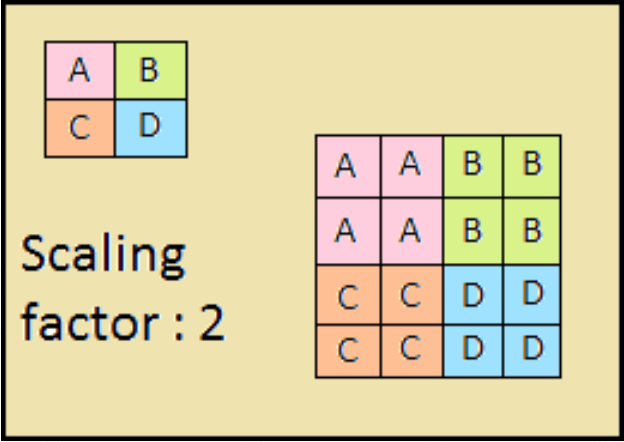
\includegraphics[width=0.8\textwidth]{upsample.png}
\end{figure}

\begin{lstlisting}
layer = nn.Conv2d(2, 16, kernel_size=3, stride=1, padding=1)
x = torch.rand(1, 2, 28, 28)
out = layer(x) #python provide magic to call __call__
out.shape   # torch.Size([1, 16, 28, 28])

out = F.interpolate(out, scale_factor=2, mode='nearest')
out.shape   # torch.Size([1, 16, 56, 56])
\end{lstlisting}


\subsubsection{ReLu}
\begin{figure}[!h]
  \centering
  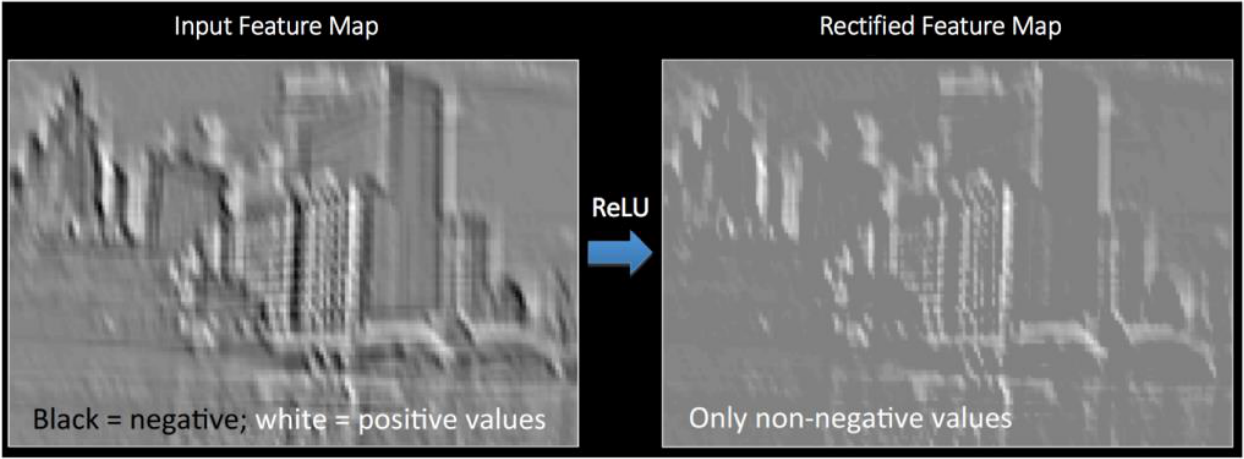
\includegraphics[width=1\textwidth]{convReLu.png}
\end{figure}

\begin{lstlisting}
layer = nn.Conv2d(2, 16, kernel_size=3, stride=1, padding=1)
x = torch.rand(1, 2, 28, 28)
out = layer(x) #python provide magic to call __call__
out.shape   # torch.Size([1, 16, 28, 28])
out.min()   # tensor(-1.2756, grad_fn=<MinBackward1>)

layer = nn.ReLU(inplace=True)
out = layer(out)
out.shape   # torch.Size([1, 16, 28, 28])
out.min()   tensor(0., grad_fn=<MinBackward1>)
\end{lstlisting}

\subsection{Batch Norm}
\textbf{Batch normalization 广泛应用于深度学习,CNN,RNN.}
\subsubsection{使用原因}
\begin{figure}[!h]
  \centering
  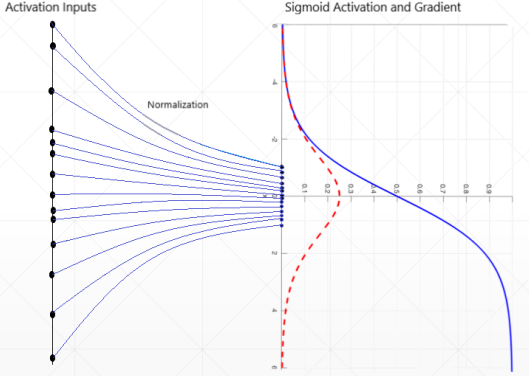
\includegraphics[width=0.6\textwidth]{BNExplanation.png}
\end{figure}

\textbf{通过 BatchNorm 极大地避免使用 Sigmoid 函数时的梯度弥散情况,加快迭代收敛速度。}

\subsubsection{Feature Scaling}
\textcolor{red}{更加利于搜索最优解。}

\textbf{1. image Normlization}
\begin{lstlisting}
normlize = transforms.Normalize(mean=[0.485, 0.456, 0.406]
                                std=[0.229, 0.224, 0.225]) #RGB
\end{lstlisting}
将输入的 image 数据,范围在 0-1 之间,经过 标准化,使其服从 N(0, 1) 分布,更利用于空间搜索最优解。

\textbf{2. Batch Normlization}\\

常见的 Norm 类型。
\begin{figure}[!h]
  \centering
  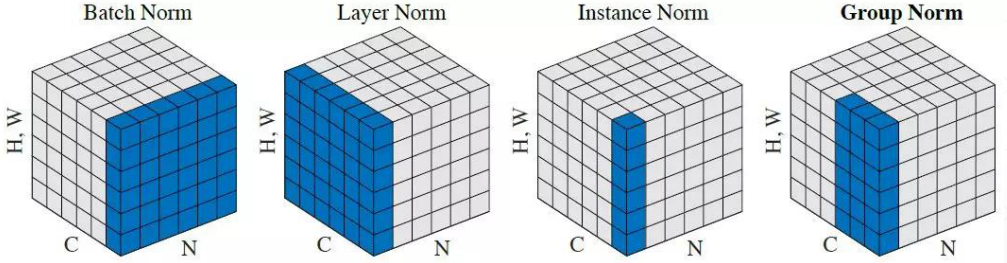
\includegraphics[width=0.8\textwidth]{BNType.png}
\end{figure}

\textbf{可以看出来 Batch Normlization 只保留 channel 的统计数据 mean 以及 varience.}
\begin{figure}[!h]
  \centering
  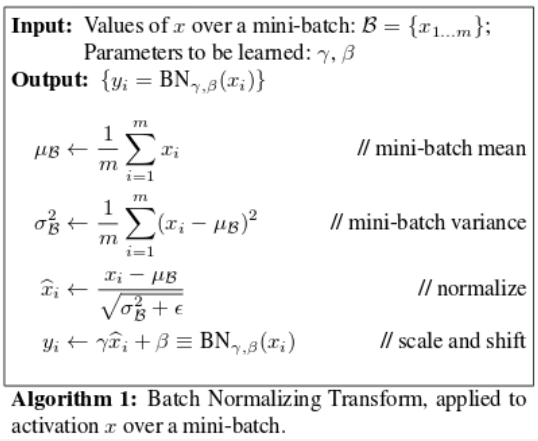
\includegraphics[width=0.6\textwidth]{BNFormula.png}
\end{figure}
\begin{figure}[!h]
  \centering
  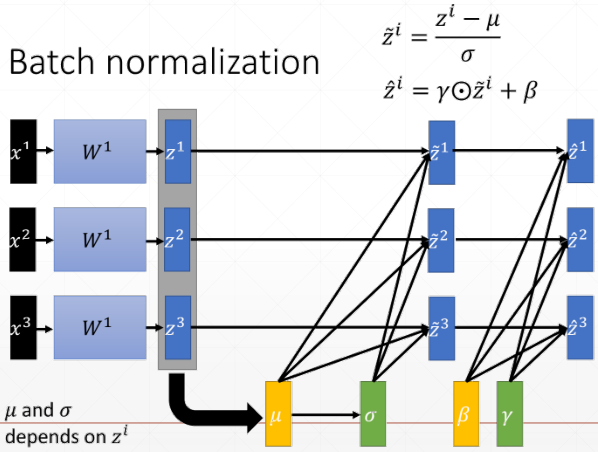
\includegraphics[width=0.6\textwidth]{BNProcess.png}
\end{figure}

\textcolor{red}{Batch Normlization 只会平移和缩放数据。}


\begin{lstlisting}
x = torch.rand(100, 16, 784)
layer = nn.BatchNorm1d(16)
out = layer(x)
out.shape   # torch.Size([100, 16, 784])
layer.running_mean.shape   # torch.Size([16])
layer.running_var.shape   # torch.Size([16])
\end{lstlisting}

\textbf{Class Variables, 查看类变量}
\begin{lstlisting}
vars(layer)
# 'affine': True,    otherwise weight=1, bias=0 not update
# 'training': True,    not test mode
\end{lstlisting}

\textbf{Batch Normlization 在 training 以及 test 行为不一样。}

\textcolor{red}{因为在test时, 数据没有 Batch 统计单个数据 没有意义,因此只会使用 全局的 mean 以及 varience .且 weight 以及 bias 是不需要更新的。}

\begin{lstlisting}
layer.eval()     # 'training': False,
hatx = torch.rand(1, 16, 7, 7)
test = layer(hatx)
\end{lstlisting}

\subsubsection{使用效果}
\begin{figure}[!h]
  \centering
  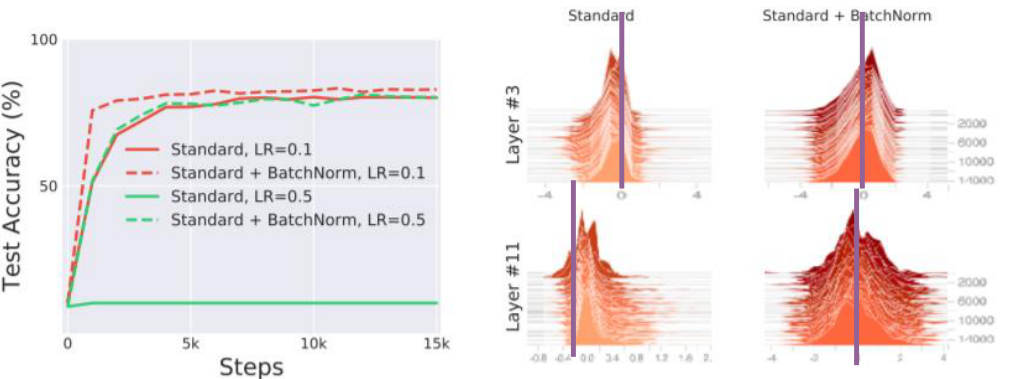
\includegraphics[width=1\textwidth]{BNVisualization.png}
\end{figure}

\subsubsection{使用优势}
\begin{enumerate}
  \item 加快收敛速度
  \item 更好的效果
  \item 模型更健壮
  \begin{itemize}
    \item 稳定性
    \item 学习率过大
  \end{itemize}
\end{enumerate}


\subsection{经典的卷积神经网络}
\subsubsection{ImageNet dataset 224x224}
\begin{figure}[!h]
  \centering
  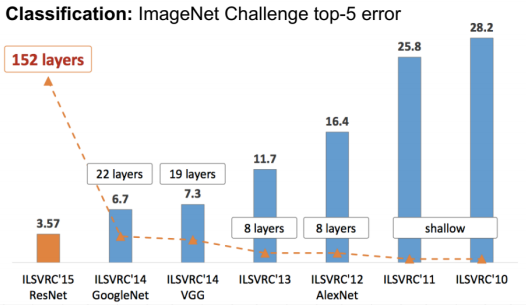
\includegraphics[width=0.7\textwidth]{popular.png}
\end{figure}

\subsubsection{LeNet-5}
\textbf{Yann LeCun 深度学习三驾马车之一}
\begin{figure}[!h]
  \centering
  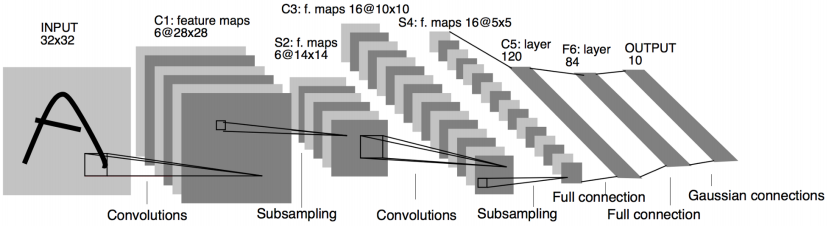
\includegraphics[width=0.8\textwidth]{LeNet5.png}
\end{figure}

上世纪80年代产物,用于手写字体识别,精度优秀。

\subsubsection{AlexNet}
\textbf{Geoffrey Hinton 深度学习三驾马车之首}

\begin{enumerate}
  \item GTX 580
    \begin{itemize}
      \item 3GB x 2
    \end{itemize}
  \item 11 x 11
  \item 8 layers
\end{enumerate}

\begin{figure}[!h]
  \centering
  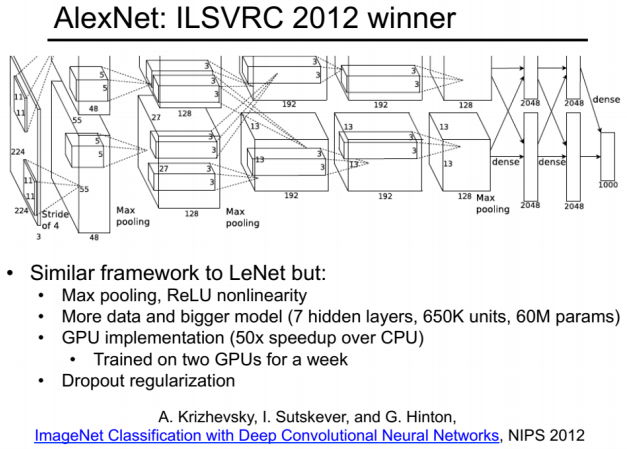
\includegraphics[width=0.8\textwidth]{AlexNet.png}
\end{figure}

\subsubsection{VGGNet}
\begin{enumerate}
  \item 3x3
  \item 1x1
  \item 11-19 layer
\end{enumerate}
\begin{figure}[!h]
  \centering
  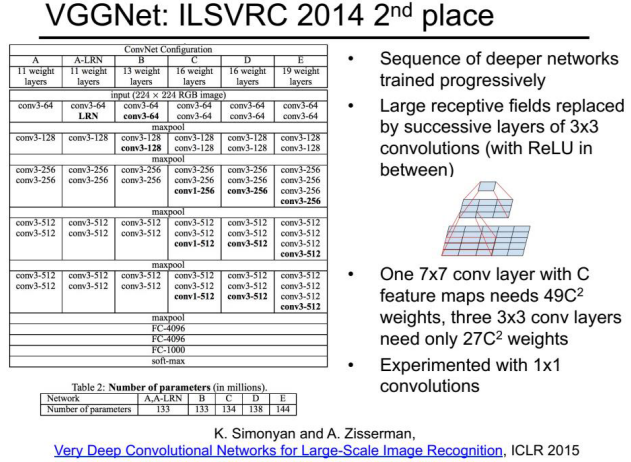
\includegraphics[width=0.8\textwidth]{VGGNet.png}
\end{figure}

\textbf{1x1 convolution}\\
1. less computation
2. c\_in $=>$ c\_out

\subsubsection{GoogLeNet}
\begin{figure}[!h]
  \centering
  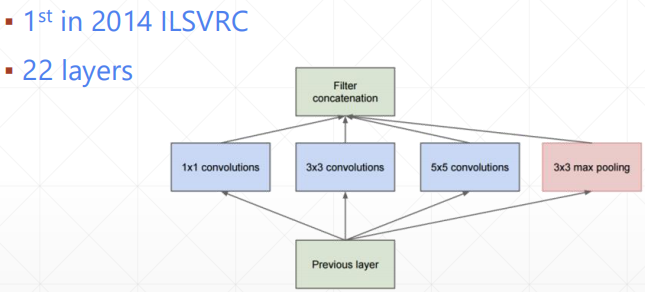
\includegraphics[width=1\textwidth]{googleNet1.png}
\end{figure}

\textbf{综合不同 size's kernel 的感受野。}

\begin{figure}[!h]
  \centering
  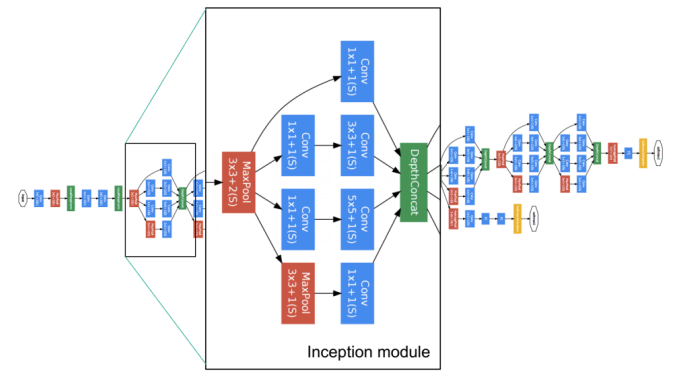
\includegraphics[width=1\textwidth]{googleNet2.png}
\end{figure}

\textcolor{red}{虽然深度学习随着网络层数的增加精度上有了明显的提升,但也不能无限制的增加网络层数,否则 training 难度增加,精度不升反降。\textbf{ResNet}}
\begin{figure}[!h]
  \centering
  \includegraphics[width=1\textwidth]{CNNLayerNumberAction.png}
\end{figure}

\subsection{ResNet}
\textbf{深度残差网络}
\begin{figure}[!h]
  \centering
  \includegraphics[width=0.8\textwidth]{ResNet1.png}
\end{figure}

\textcolor{red}{提出短路层,寻找梯度回传的捷径。将新的 Unit 进行叠加形成 ResNet.}

\begin{figure}[!h]
  \centering
  \includegraphics[width=0.8\textwidth]{ResNet2.png}
\end{figure}

\textcolor{red}{新的 Unit 单元,shape 不能变。将短路权利交给网络。}

\begin{figure}[!h]
  \centering
  \includegraphics[width=0.8\textwidth]{Boom.png}
\end{figure}

\textbf{\textcolor{red}{为什么叫残差(Residual)?}}
\begin{figure}[!h]
  \centering
  \includegraphics[width=0.5\textwidth]{residual.png}
\end{figure}

层数性能比较:
\begin{figure}[!h]
  \centering
  \includegraphics[width=1\textwidth]{NetCompare.png}
\end{figure}

\newpage
\subsection{DenseNet}
\begin{figure}[!h]
  \centering
  \includegraphics[width=1\textwidth]{DenseNet.png}
\end{figure}

\subsection{nn.Module}
\textbf{当我们自己定义网络层时,必须继承 nn.Module 父类。常用的线性层,卷积层等 PyTorch 官方已经写好。}
\begin{lstlisting}
class MyLinear(nn.Module):

    def __init__(self, inp, outp):
        super(MyLinear, self).__init__()

        # requires_grad = True
        self.w = nn.Parameter(torch.randn(outp, inp))
        self.b = nn.Parameter(torch.randn(outp))

    def forward(self, x):
        x = x @ self.w.t() + self.b
        return x
\end{lstlisting}

\textbf{Magic}
\begin{enumerate}
  \item Every Layer is nn.Module
  \begin{itemize}
    \item nn.Linear
    \item nn.BatchNorm2d
    \item nn.Conv2d
  \end{itemize}
  \item nn.Module is nested in nn.Module
\end{enumerate}

\textbf{使用 nn.Module 的好处}
\begin{enumerate}
  \item 可以使用大量现成的网络层。
  \begin{itemize}
    \item Linear
    \item ReLu
    \item Sigmoid
    \item Conv2d
    \item ConvTransposed2d
    \item Dropout
    \item etc.
  \end{itemize}
  \item Container 容器
  \begin{itemize}
    \item net(x)
  \end{itemize}
  \begin{lstlisting}
  self.model = nn.Sequential(
            nn.Linear(784, 200),
            nn.LeakyReLU(inplace=True),
            nn.Linear(200, 200),
            nn.LeakyReLU(inplace=True),
            nn.Linear(200, 10),
            nn.LeakyReLU(inplace=True),
        )
  \end{lstlisting}
  \item 有效管理参数
  \begin{lstlisting}
  net.parameters()   # iterator
  net.named_parameters   # auto-named weight and bias  iterator
  \end{lstlisting}
  \item Modules
  \begin{itemize}
    \item modules: all nodes
    \item children: direct children
  \end{itemize}
  \begin{lstlisting}
  class Net(nn.Module):

    def __init__(self):
        super(Net, self).__init__()

        self.net = nn.Sequential(BasicNet(),
                                 nn.ReLU(),
                                 nn.Linear(3, 2))

    def forward(self, x):
        return self.net(x)


modules: net Sequential(
(0): BasicNet(
    (net): Linear(in_features=4, out_features=3, bias=True)
    )
(1): ReLU()
(2): Linear(in_features=3, out_features=2, bias=True)
)

modules: net.0 BasicNet(
              (net): Linear(in_features=4, out_features=3, bias=True)
               )
modules: net.0.net Linear(in_features=4, out_features=3, bias=True)

modules: net.1 ReLU()
modules: net.2 Linear(in_features=3, out_features=2, bias=True)
  \end{lstlisting}
  \item GPU 加速
  \begin{lstlisting}
  device = torch.device('cuda')
  net = Net()
  net.to(device)
  \end{lstlisting}

  \item 保存与加载中间数据
  \begin{lstlisting}
  net.load_state_dict(torch.load('ckpt.mdl'))
  ...train...
  torch.save(net.state_dict(), 'ckpt.mdl')
  \end{lstlisting}

  \item train\&test 状态切换方便。
  \begin{lstlisting}
  # train
  net.train()
  ...
  # test
  net.eval()
  \end{lstlisting}
      \item 实现我们自己的类。
  \begin{lstlisting}
class Flatten(nn.Module):

    def __init__(self):
        super(Flatten, self).__init__()

    def forward(self, input):
        return input.view(input.size(0), -1)

class TestNet(nn.Module):

    def __init__(self):
        super(TestNet, self).__init__()

        self.net = nn.Sequential(nn.Conv2d(1, 16, stride=1, padding=1),
                                 nn.MaxPool2d(2, 2),
                                 Flatten(),
                                 nn.Linear(1*14*14, 10))

def forward(self, x):
        return self.net(x)
    \end{lstlisting}

    \item 自己实现的线性层
    \begin{lstlisting}
    class MyLinear(nn.Module):

    def __init__(self, inp, outp):
        super(MyLinear, self).__init__()

        # requires_grad = True
        self.w = nn.Parameter(torch.randn(outp, inp))
        self.b = nn.Parameter(torch.randn(outp))

    def forward(self, x):
        x = x @ self.w.t() + self.b
        return x
    \end{lstlisting}

\end{enumerate}



\subsection{数据增强}
\textbf{确保深度学习的深度网络有良好的表现,防止过拟合的重要标准就是要使用的是大数据集。}

\noindent\textbf{数据量小时训练技巧}
\begin{enumerate}
  \item Small network capacity.
  \item Regularization.
  \item data argumentation.
\end{enumerate}

\noindent\textbf{Data Argumentation}
\begin{enumerate}
  \item Flip 翻转
  \item Rotation 旋转
  \item scale 缩放
  \item Random Move \& Crop  平移\&缩放
  \item GAN 生成对抗网络
\end{enumerate}
\subsubsection{Flip}
\begin{figure}[!h]
  \centering
  \includegraphics[width=0.82\textwidth]{flip.png}
\end{figure}

\begin{lstlisting}
train_loader = torch.utils.data.DataLoader(
    datasets.MNIST('../data', train=True, download=True,
                   transform=transforms.Compose([
                       transforms.RandomHorizontalFlip(),
                       transforms.RandomVerticalFlip(),
                   ])),
\end{lstlisting}
\newpage
\subsubsection{Rotation}
\begin{figure}[!h]
  \centering
  \includegraphics[width=1\textwidth]{rotation.png}
\end{figure}

\begin{lstlisting}
train_loader = torch.utils.data.DataLoader(
    datasets.MNIST('../data', train=True, download=True,
                   transform=transforms.Compose([
                       transforms.RandomRotation(15),
                       transforms.RandomRotation([90, 180, 270]),
                   ]))
\end{lstlisting}

\subsubsection{Scale}
\begin{figure}[!h]
  \centering
  \includegraphics[width=0.82\textwidth]{scale.png}
\end{figure}

\begin{lstlisting}
train_loader = torch.utils.data.DataLoader(
    datasets.MNIST('../data', train=True, download=True,
                   transform=transforms.Compose([
                       transforms.Resize([32, 32]),
                   ])),
\end{lstlisting}


\subsubsection{crop part}
\begin{figure}[!h]
  \centering
  \includegraphics[width=0.82\textwidth]{crop.png}
\end{figure}

\begin{lstlisting}
train_loader = torch.utils.data.DataLoader(
    datasets.MNIST('../data', train=True, download=True,
                   transform=transforms.Compose([
                       transforms.RandomCrop([28, 28]),
                   ])),
\end{lstlisting}

\subsubsection{noise}
\begin{figure}[!h]
  \centering
  \includegraphics[width=0.82\textwidth]{noise.png}
\end{figure}

\textbf{pytorch 没有 加入高斯白噪点的 API,可人为加上高斯分布图片实现 图片的随机噪声。}





























%\newpage
%\begin{figure}[!h]
%  \centering
%  \includegraphics[width=0.9\textwidth]{PyTorch.png}
%  \caption{大纲图}
%\end{figure}
%\newpage

